\documentclass[12pt,a4paper]{article}
\usepackage{natbib}
\usepackage{graphicx}
\usepackage{float}
\usepackage{multirow}
\usepackage{multicol}
\usepackage{subfig}
\usepackage{alphalph}
\usepackage{scrextend}
\usepackage{xcolor}
\renewcommand\thesubfigure{\alphalph{\value{subfigure}}}

\begin{document}
\title{Pulsar detection - Machine learning and pattern recognition exam}
\author{Alberto Baroso \\ s296520}
\vspace{1cm}
\date{2023-01-31}
\maketitle
\clearpage

\begin{abstract}
    The Pulsar dataset \cite{stw656} is a collection of 17.898 pulsar candidates of which 1.639 are real pulsars and 16,259 are spurious examples caused by RFI/noise.
    A pulsar is a neutron star that emits beams of electromagnetic radiation.
    As pulsars rotate, their emission beam sweeps across the sky, a periodically repeated pattern of broadband radio emission can be detected as this beam crosses our line of sight.
    Thus pulsar search involves looking for periodic radio signals with large radio telescopes.
    \\ \\
    The goal of this project is to find the best machine learning techniques to solve the binary classification problem of detecting pulsars from the Pulsar dataset.
    The analysis starts with the exploration of the dataset and its features, it proceeds with the application of dimensionality reduction and preprocessing techniques,
    different kinds of models are then evaluated and their scores are calibrated, finally, experiments are carried out on the test dataset to evaluate if the choices made during training were optimal.
\end{abstract}
\clearpage

\tableofcontents
\clearpage

\section{Problem analysis}

\subsection{Datasets}

The Pulsar dataset \cite{stw656} contains 17.898 pulsar candidates of which 1.639 are real pulsars and 16,259 are spurious examples.
The distribution of the two classes is highly unbalanced.
The data has been split into a training set and a test set:
\begin{itemize}
    \item The training set contains 8929 samples, of which 8108 are non-pulsars and 821 are pulsars.
    \item The test set contains 8969 samples, of which 8151 are non-pulsars and 818 are pulsars.
\end{itemize}
The class labels used are: 0 for non-pulsar samples and 1 for pulsars.

\subsection{Feature descriptions}

Pulsar candidates are described by 8 continuous features extracted from radio signals collected by radio telescopes.
The first four are simple statistics obtained from the integrated pulse profile (folded profile).
This is an array of continuous features that describe a longitude-resolved version of the signal that has been averaged in both time and frequency (see \cite{Lyon2016} for more details).
The remaining four features are similarly obtained from the DM-SNR curve (again see \cite{Lyon2016} for more details).
The features are listed below:

\begin{enumerate}
    \item Mean of the integrated profile.
    \item Standard deviation of the integrated profile.
    \item Excess kurtosis of the integrated profile.
    \item Skewness of the integrated profile.
    \item Mean of the DM-SNR curve.
    \item Standard deviation of the DM-SNR curve.
    \item Excess kurtosis of the DM-SNR curve.
    \item Skewness of the DM-SNR curve.
\end{enumerate}

\subsection{Feature distributions and ranges}

\begin{figure}[H]
    \begin{center}
        \begin{tabular}{cc}
            \subfloat[]{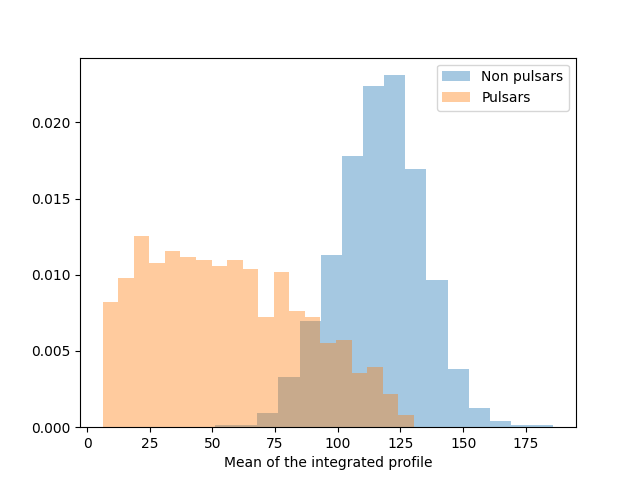
\includegraphics[width = 183pt, height = 120pt]{img/unprocessed_feature_distributions/mean_of_ip.png}}                &
            \subfloat[]{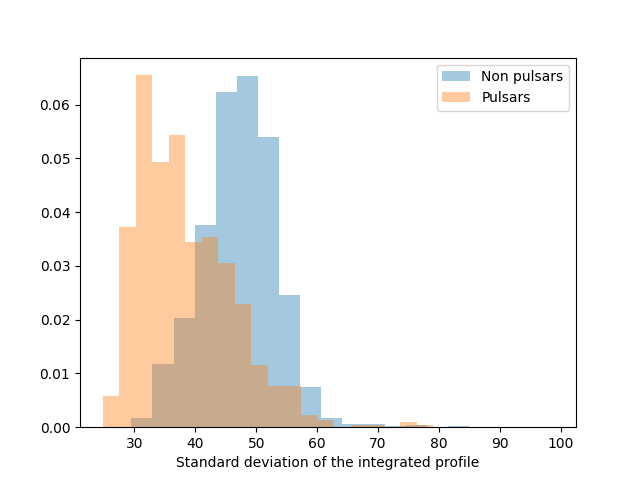
\includegraphics[width = 183pt, height = 120pt]{img/unprocessed_feature_distributions/stdev_of_ip.png}}                 \\
            \subfloat[]{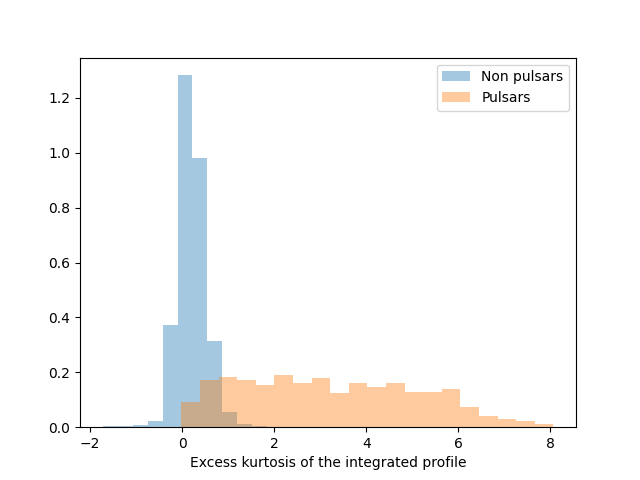
\includegraphics[width = 183pt, height = 120pt]{img/unprocessed_feature_distributions/excess_kurtosis_of_ip.png}}     &
            \subfloat[]{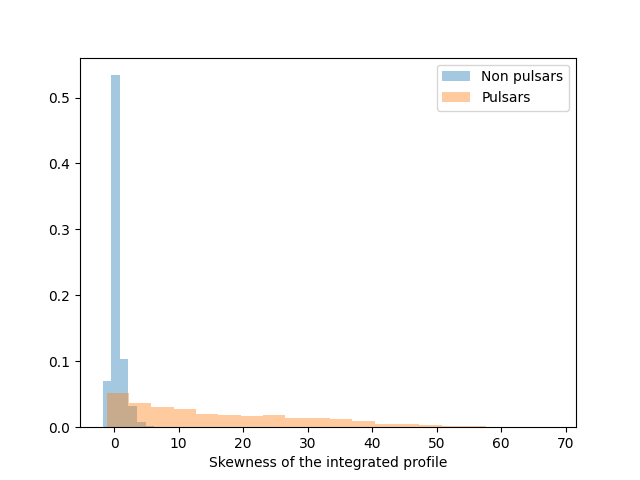
\includegraphics[width = 183pt, height = 120pt]{img/unprocessed_feature_distributions/skewness_of_ip.png}}              \\
            \subfloat[]{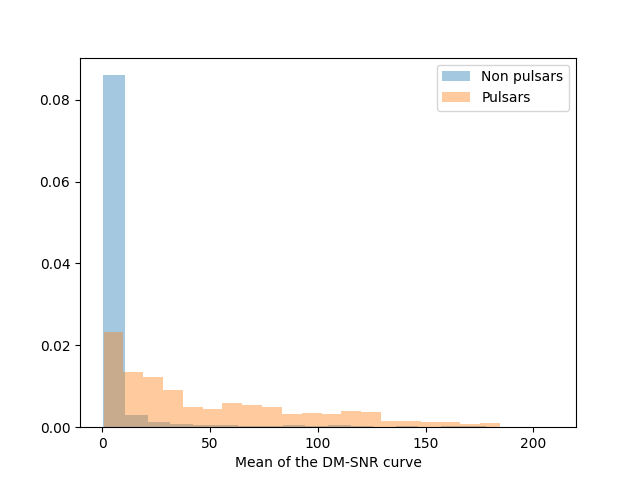
\includegraphics[width = 183pt, height = 120pt]{img/unprocessed_feature_distributions/mean_of_dm-snr.png}}            &
            \subfloat[]{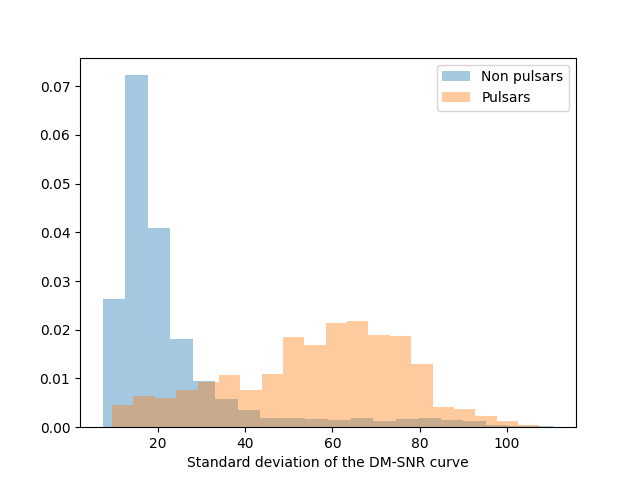
\includegraphics[width = 183pt, height = 120pt]{img/unprocessed_feature_distributions/stdev_of_dm-snr.png}}             \\
            \subfloat[]{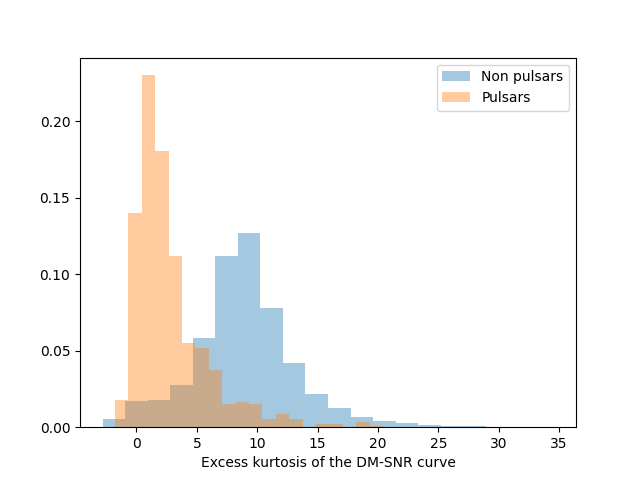
\includegraphics[width = 183pt, height = 120pt]{img/unprocessed_feature_distributions/excess_kurtosis_of_dm-snr.png}} &
            \subfloat[]{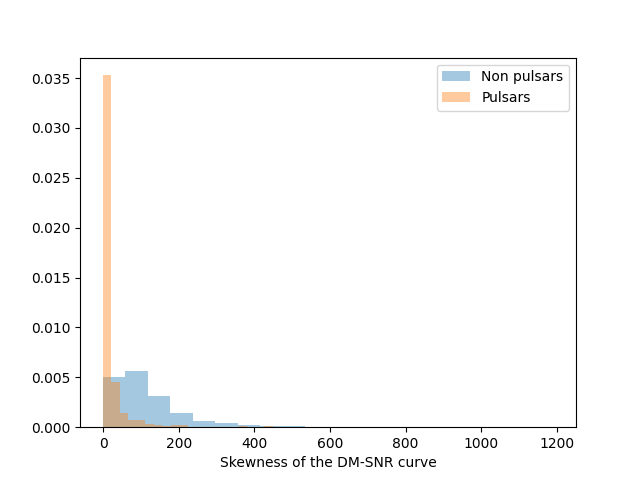
\includegraphics[width = 183pt, height = 120pt]{img/unprocessed_feature_distributions/skewness_of_dm-snr.png}}          \\
        \end{tabular}
    \end{center}
\end{figure}

\begin{minipage}{\linewidth}
    \begin{tabular}{ |c|p{220pt}|p{34pt}|p{30pt}|p{36pt}|  }\hline

           & Feature                                      & Mean   & Min   & Max     \\
        \hline
        a. & Mean of the integrated profile               & 110.86 & 6.18  & 186.02  \\
        \hline
        b. & Standard deviation of the integrated profile & 46.47  & 24.77 & 98.78   \\
        \hline
        c. & Excess kurtosis of the integrated profile    & 0.49   & -1.73 & 8.07    \\
        \hline
        d. & Skewness of the integrated profile           & 1.84   & -1.79 & 68.10   \\
        \hline
        e. & Mean of the DM-SNR curve                     & 12.67  & 0.21  & 209.30  \\
        \hline
        f. & Standard deviation of the DM-SNR curve       & 26.25  & 7.37  & 110.64  \\
        \hline
        g. & Excess kurtosis of the DM-SNR curve          & 8.33   & -2.81 & 34.54   \\
        \hline
        h. & Skewness of the DM-SNR curve                 & 105.41 & -1.98 & 1191.00 \\
        \hline
    \end{tabular}
    \captionof{table}{Feature ranges}
\end{minipage}
\vspace{1cm}

An initial analysis of the raw features of the training data shows that:
\begin{itemize}
    \item Features mainly follow irregular distributions
    \item Few features, the ones for non-pulsars in figures (a), (b), and (g), present distributions similar to Gaussians
    \item Looking at graph (b) it's possible to deduce that the "Standard Deviation of the integrated profile" could be one of the less informative features as the histograms of the two classes share one of the largest overlapping areas compared to the other graphs. But since it also has a good amount of non-overlapping areas it can still provide useful information for classification purposes.
    \item Graphs (c) and (d) show that "Excess of kurtosis of integrated profile" and "Skewness of integrated profile" could be among the best features for sample discrimination, as they have little overlapping areas of the histograms.
    \item Values for non-pulsars are generally concentrated around some values, while pulsars present a wider range of values.
    \item Some features, mainly the ones in graphs (b), (d), and (h), are characterized by the presence of significantly large outliers. Similar claims can be made by looking at the ranges of minimum and maximum values for the corresponding features. It's possible to expect classification algorithms to provide less than ideal results due to the presence of outliers.
\end{itemize}

\subsection{Feature correlation}

\begin{figure}[H]
    \begin{center}
        \begin{tabular}{ccc}
            \hspace*{-65pt}
            \subfloat[]{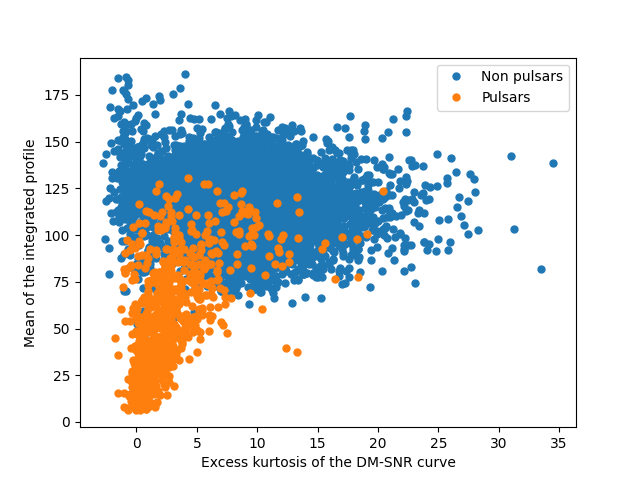
\includegraphics[width = 160pt]{img/unprocessed_feature_pairs/mean_ip-excess_kurtosis_dm-snr.png}} &
            \subfloat[]{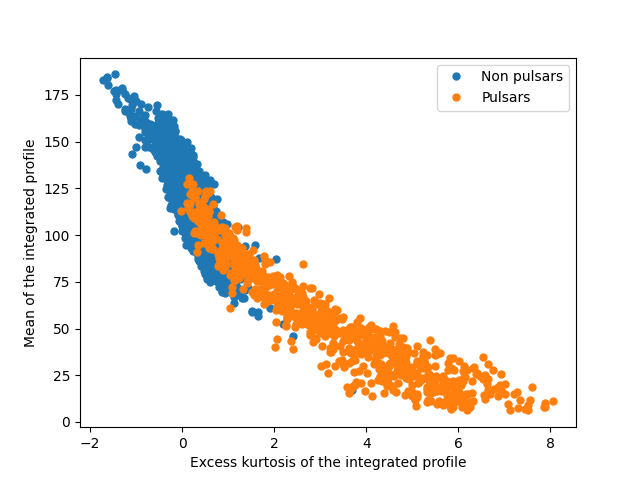
\includegraphics[width = 160pt]{img/unprocessed_feature_pairs/mean_ip-excess_kurtosis_ip.png}}     &
            \subfloat[]{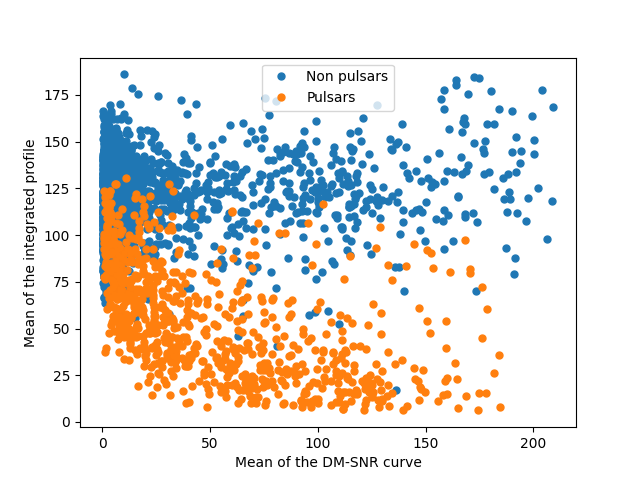
\includegraphics[width = 160pt]{img/unprocessed_feature_pairs/mean_ip-mean_dm-snr.png}}              \\
            \hspace*{-65pt}
            \subfloat[]{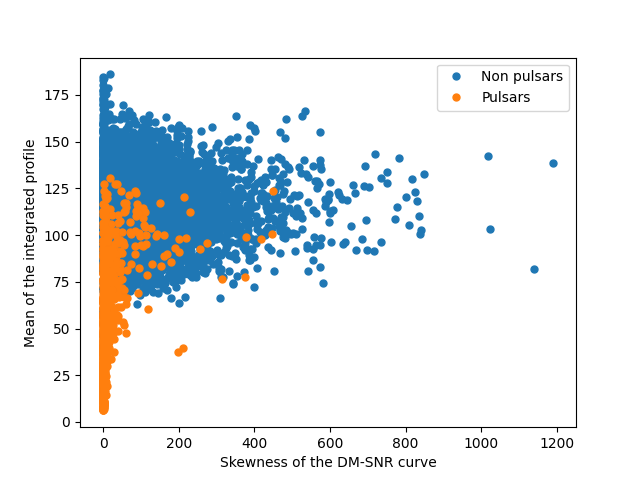
\includegraphics[width = 160pt]{img/unprocessed_feature_pairs/mean_ip-skewness_dm-snr.png}}        &
            \subfloat[]{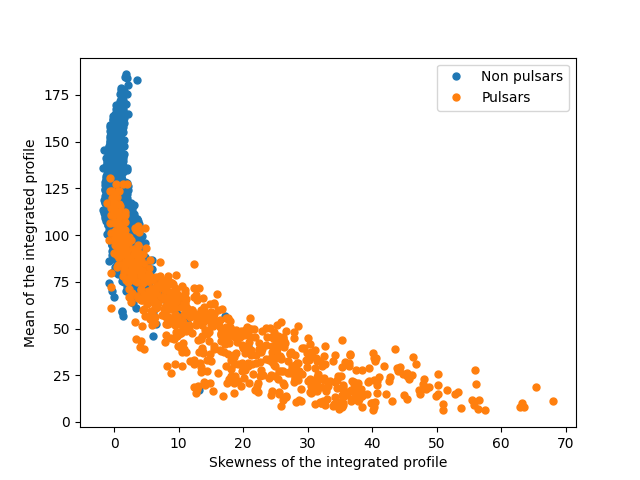
\includegraphics[width = 160pt]{img/unprocessed_feature_pairs/mean_ip-skewness_ip.png}}            &
            \subfloat[]{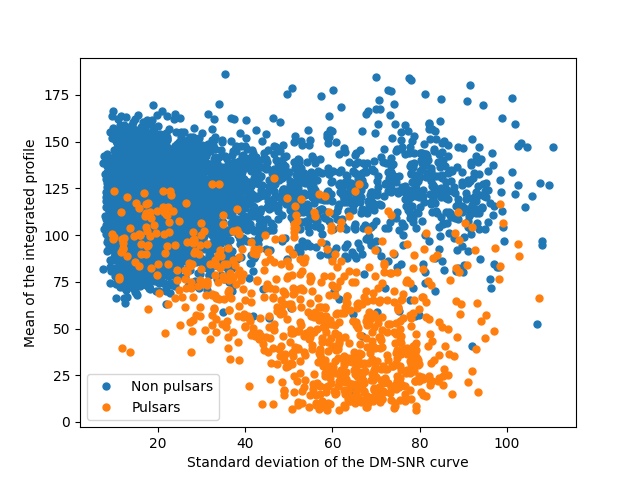
\includegraphics[width = 160pt]{img/unprocessed_feature_pairs/mean_ip-stdev_dm-snr.png}}             \\
            \hspace*{-65pt}
            \subfloat[]{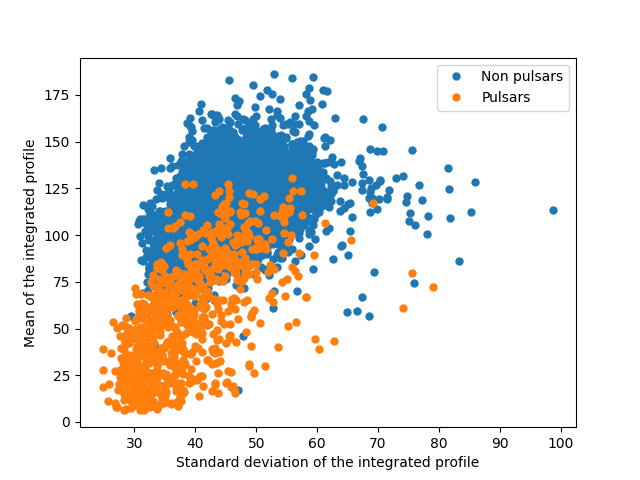
\includegraphics[width = 160pt]{img/unprocessed_feature_pairs/mean_ip-stdev_ip.png}}               &
            \subfloat[]{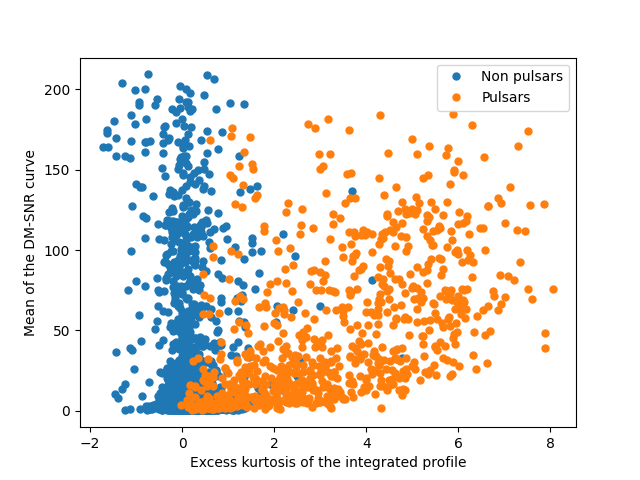
\includegraphics[width = 160pt]{img/unprocessed_feature_pairs/mean_dm-snr-excess_kurtosis_ip.png}} &
            \subfloat[]{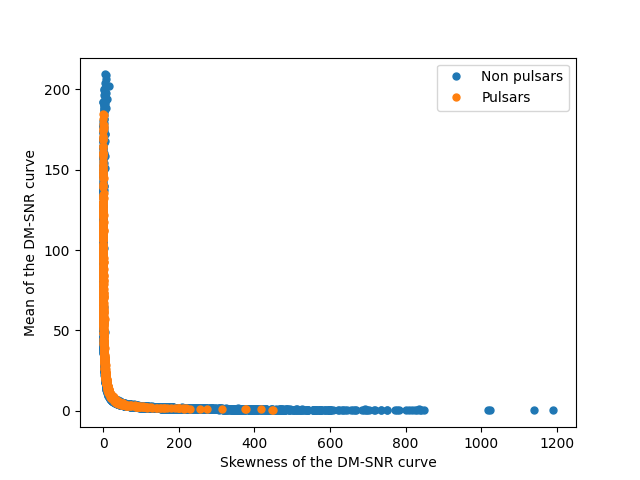
\includegraphics[width = 160pt]{img/unprocessed_feature_pairs/mean_dm-snr-skewness_dm-snr.png}}      \\
            \hspace*{-65pt}
            \subfloat[]{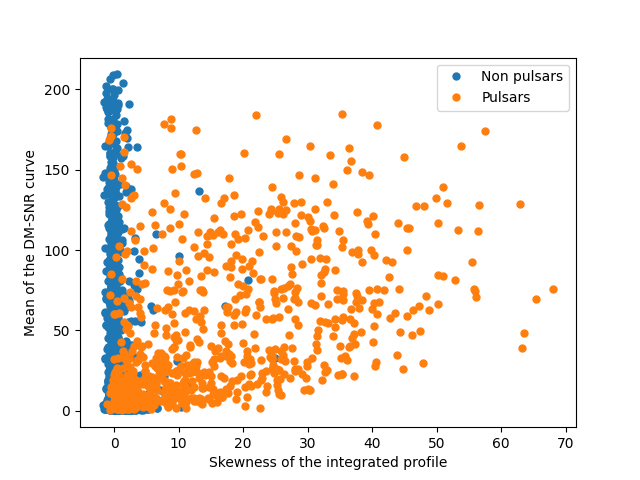
\includegraphics[width = 160pt]{img/unprocessed_feature_pairs/mean_dm-snr-skewness_ip.png}}        &
            \subfloat[]{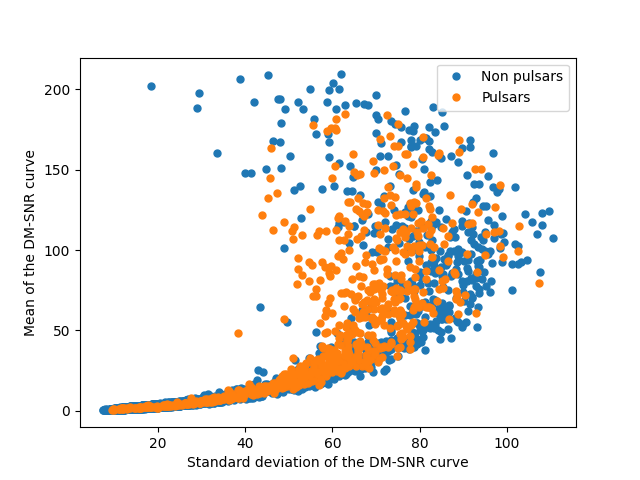
\includegraphics[width = 160pt]{img/unprocessed_feature_pairs/mean_dm-snr-stdev_dm-snr.png}}       &
            \subfloat[]{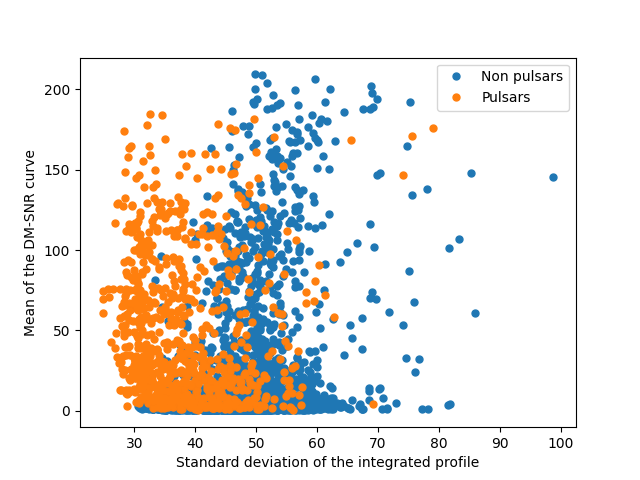
\includegraphics[width = 160pt]{img/unprocessed_feature_pairs/mean_dm-snr-stdev_ip.png}}             \\
        \end{tabular}
    \end{center}
\end{figure}
\begin{figure}[H]
    \begin{center}
        \begin{tabular}{ccc}
            \hspace*{-65pt}
            \subfloat[]{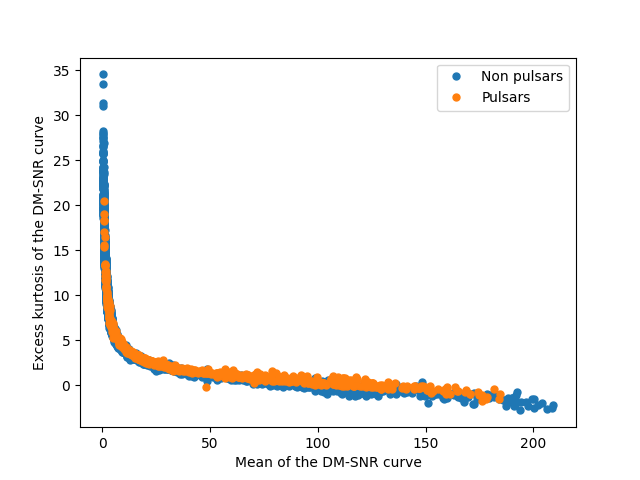
\includegraphics[width = 160pt]{img/unprocessed_feature_pairs/excess_kurtosis_dm-snr-mean_dm-snr.png}}        &
            \subfloat[]{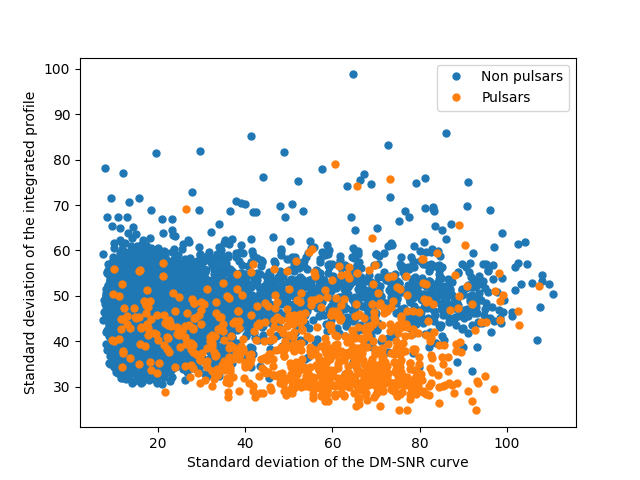
\includegraphics[width = 160pt]{img/unprocessed_feature_pairs/stdev_ip-stdev_dm-snr.png}}                     &
            \subfloat[]{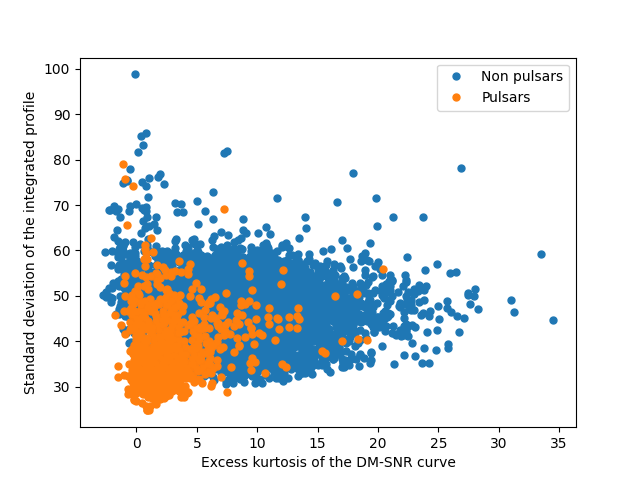
\includegraphics[width = 160pt]{img/unprocessed_feature_pairs/stdev_ip-excess_kurtosis_dm-snr.png}}             \\
            \hspace*{-65pt}
            \subfloat[]{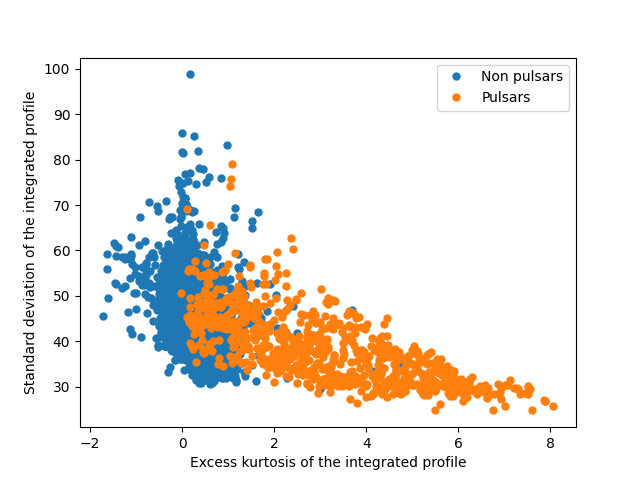
\includegraphics[width = 160pt]{img/unprocessed_feature_pairs/stdev_ip-excess_kurtosis_ip.png}}               &
            \subfloat[]{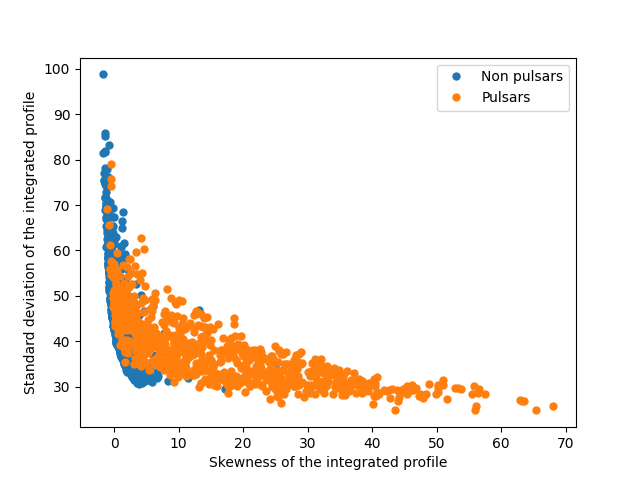
\includegraphics[width = 160pt]{img/unprocessed_feature_pairs/stdev_ip-skewness_ip.png}}                      &
            \subfloat[]{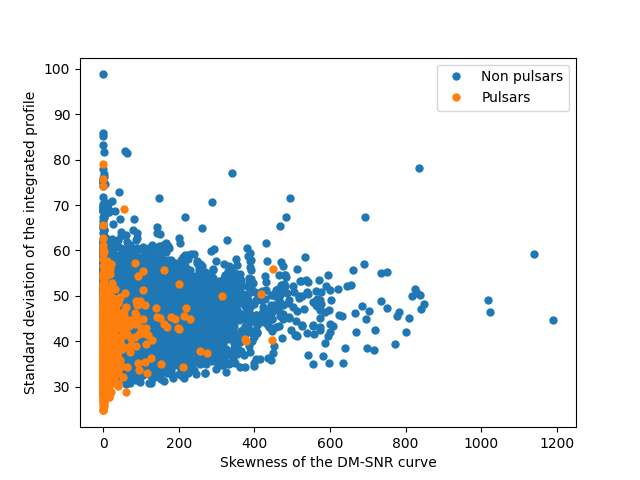
\includegraphics[width = 160pt]{img/unprocessed_feature_pairs/stdev_ip-skewness_dm-snr.png}}                    \\
            \hspace*{-65pt}
            \subfloat[]{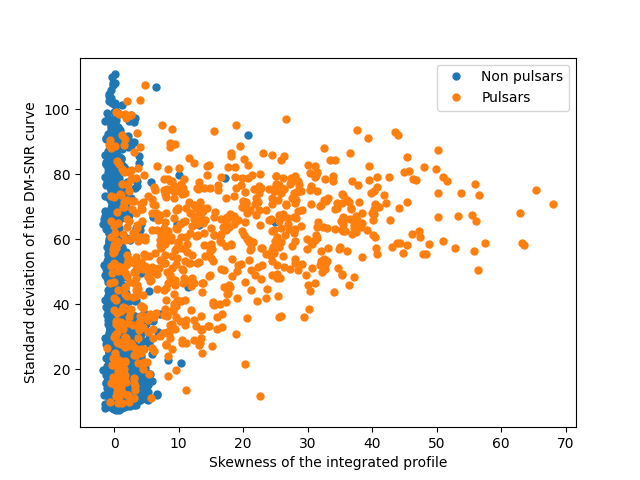
\includegraphics[width = 160pt]{img/unprocessed_feature_pairs/stdev_dm-snr-skewness_ip.png}}                  &
            \subfloat[]{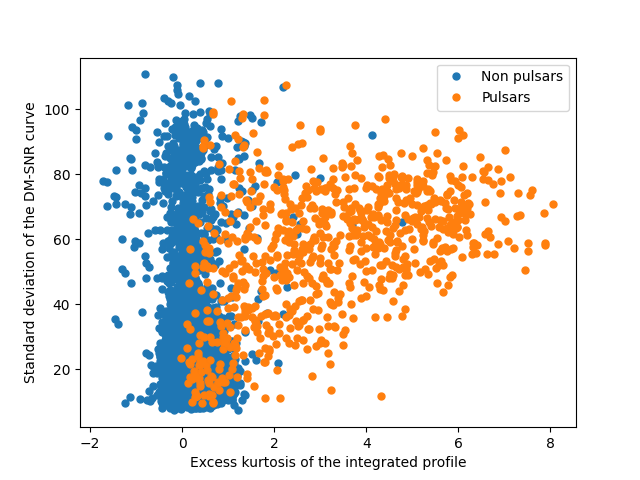
\includegraphics[width = 160pt]{img/unprocessed_feature_pairs/stdev_dm-snr-excess_kurtosis_ip.png}}           &
            \subfloat[]{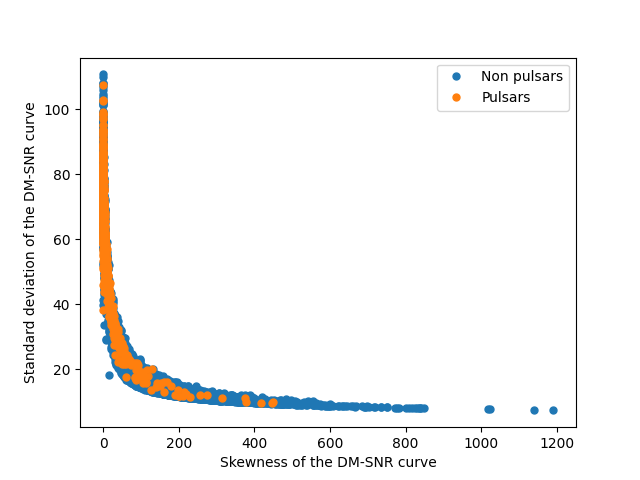
\includegraphics[width = 160pt]{img/unprocessed_feature_pairs/stdev_dm-snr-skewness_dm-snr.png}}                \\
            \hspace*{-65pt}
            \subfloat[]{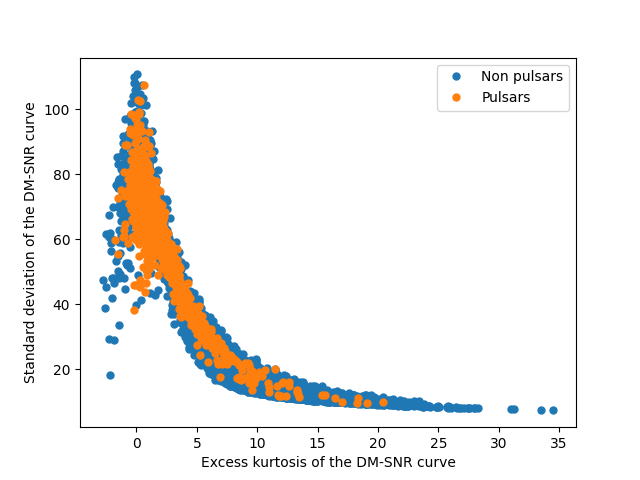
\includegraphics[width = 160pt]{img/unprocessed_feature_pairs/stdev_dm-snr-excess_kurtosis_dm-snr.png}}       &
            \subfloat[]{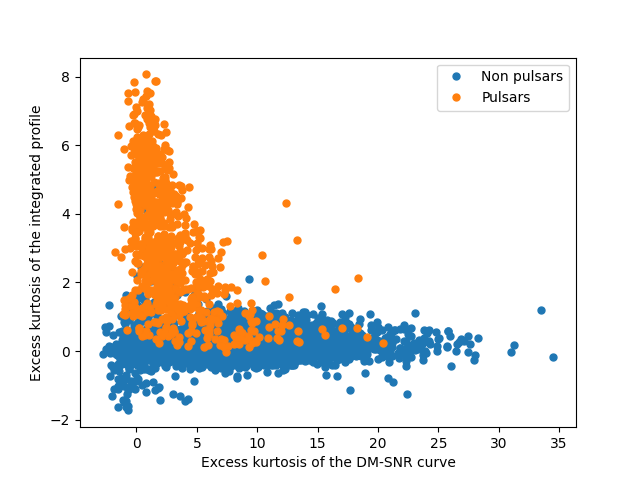
\includegraphics[width = 160pt]{img/unprocessed_feature_pairs/excess_kurtosis_ip-excess_kurtosis_dm-snr.png}} &
            \subfloat[]{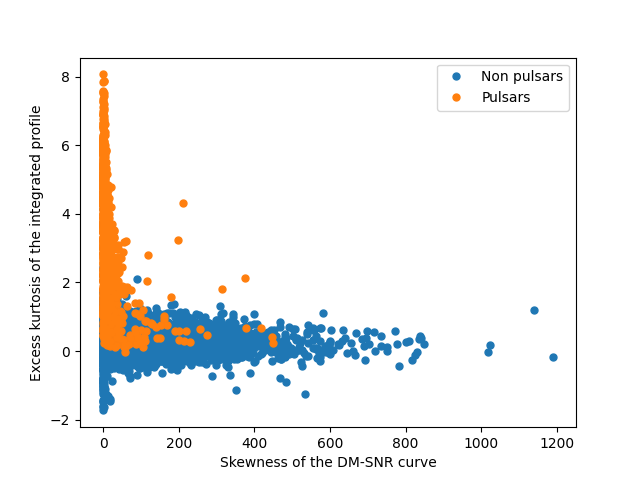
\includegraphics[width = 160pt]{img/unprocessed_feature_pairs/excess_kurtosis_ip-skewness_dm-snr.png}}          \\
        \end{tabular}
    \end{center}
\end{figure}

\begin{figure}
    \begin{center}
        \hspace*{-65pt}
        \begin{tabular}{ccc}
            \subfloat[]{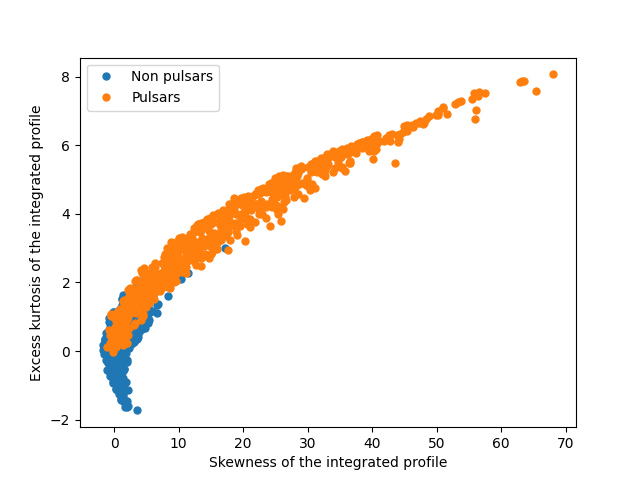
\includegraphics[width = 160pt]{img/unprocessed_feature_pairs/excess_kurtosis_ip-skewness_ip.png}}            &
            \subfloat[]{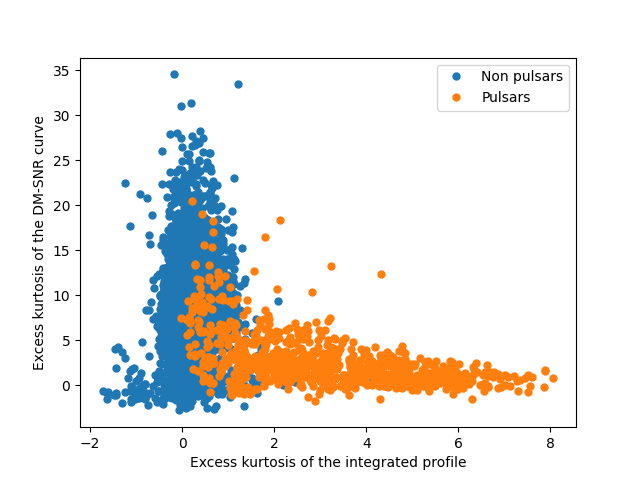
\includegraphics[width = 160pt]{img/unprocessed_feature_pairs/excess_kurtosis_dm-snr-excess_kurtosis_ip.png}} &
            \subfloat[]{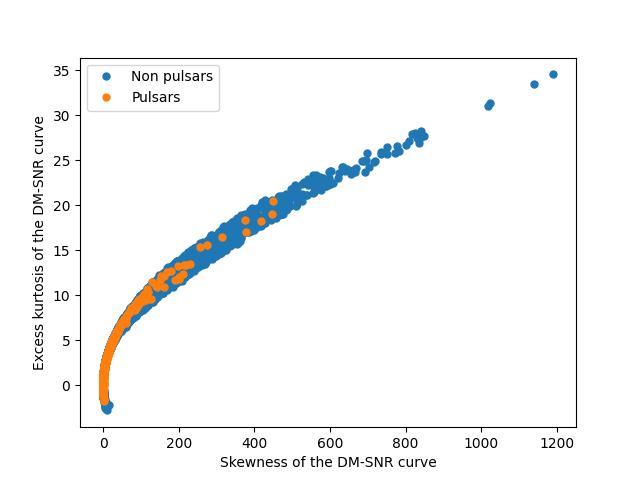
\includegraphics[width = 160pt]{img/unprocessed_feature_pairs/excess_kurtosis_dm-snr-skewness_dm-snr.png}}      \\
            \subfloat[]{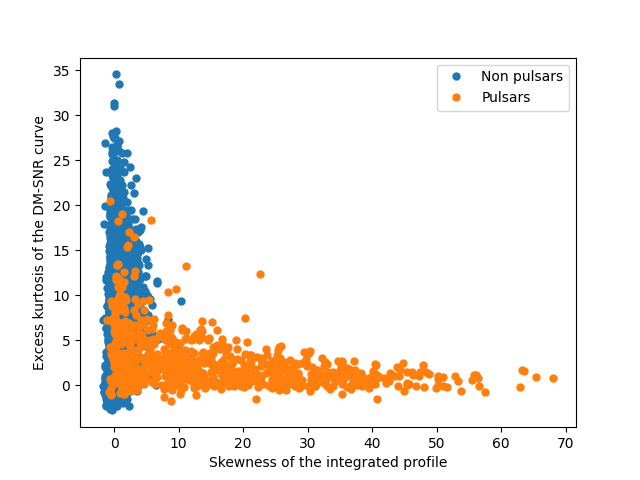
\includegraphics[width = 160pt]{img/unprocessed_feature_pairs/excess_kurtosis_dm-snr-skewness_ip.png}}        &
            \subfloat[]{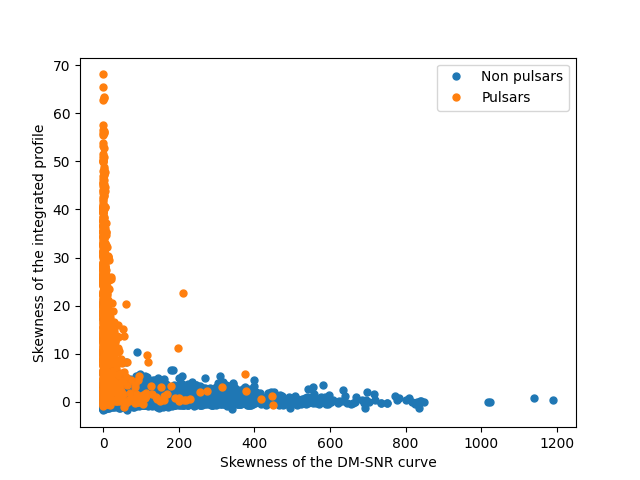
\includegraphics[width = 160pt]{img/unprocessed_feature_pairs/skewness_ip-skewness_dm-snr.png}}                 \\
        \end{tabular}
    \end{center}
\end{figure}

Observing the feature pairs it's possible to note that there isn't one that allows finding a clear separation of the two classes. \\ \\
The combination of features represented in graphs (n), (p), (ab), (af), and (ah) get close to identifying regions of space where samples are well separated. \\ \\
The least useful pairs of features are represented in graphs (q), (s), (u), and (ac), where samples are almost entirely overlapping. \\ \\
The plots also show that some pairs of features share similar distributions, implying that there is some sort of correlation between them. \\ \\
Overall, it's reasonable to believe that there are enough pairs of features that separate classes well enough to obtain good accuracy for the trained models.

\clearpage

Pearson correlation \( \frac{Cov(X,Y)}{\sqrt{Var(X)}\sqrt{Var(Y)}} \) was used to explore the correlation between all pairs of features.
The absolute value of the Pearson correlation between all pairs of features is shown in the following heatmaps: \\

\begin{figure}[H]
    \caption{Pearson correlation heatmap - RAW features}
    \begin{center}
        \begin{tabular}{ccc}
            \hspace*{-65pt}
            \subfloat[Whole dataset]{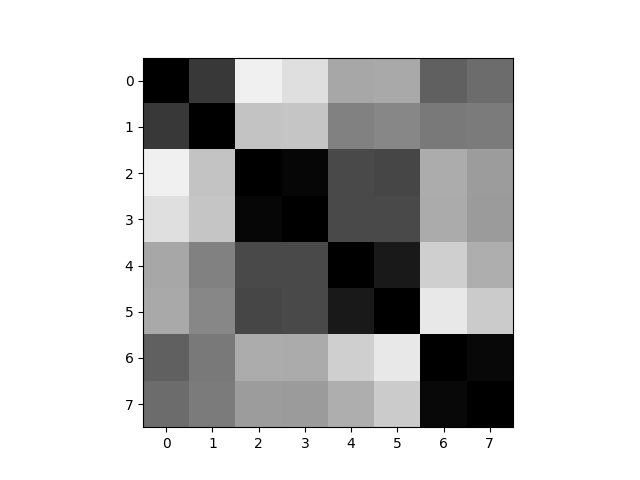
\includegraphics[width = 160pt]{img/pearson_correlation/raw_heatmap.png}}  &
            \subfloat[Pulsars]{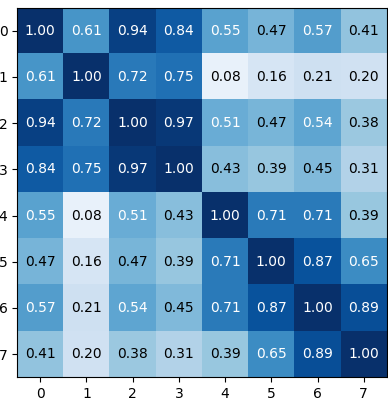
\includegraphics[width = 160pt]{img/pearson_correlation/raw_pulsar_heatmap.png}} &
            \subfloat[Non-pulsars]{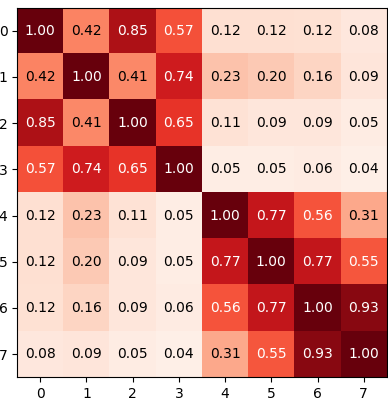
\includegraphics[width = 160pt]{img/pearson_correlation/raw_non_pulsar_heatmap.png}} \\
        \end{tabular}
    \end{center}
\end{figure}

\begin{figure}[H]
    \caption{Pearson correlation heatmap - Z-normalized features}
    \begin{center}
        \begin{tabular}{ccc}
            \hspace*{-65pt}
            \subfloat[Whole dataset]{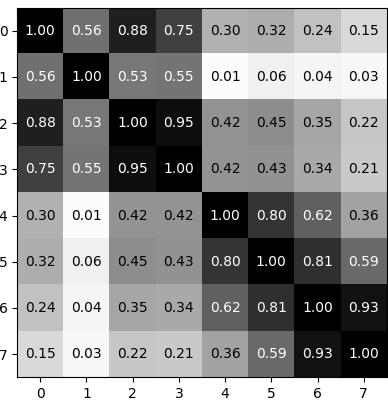
\includegraphics[width = 160pt]{img/pearson_correlation/z-normalization_heatmap.png}} &
            \subfloat[Pulsars]{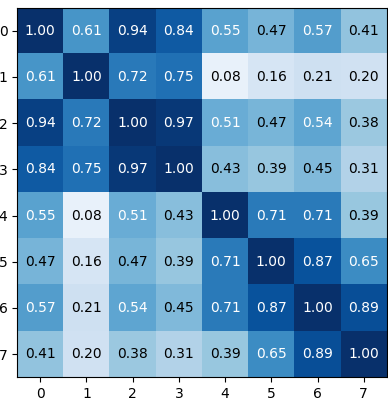
\includegraphics[width = 160pt]{img/pearson_correlation/z-normalization_pulsar.png}}        &
            \subfloat[Non-pulsars]{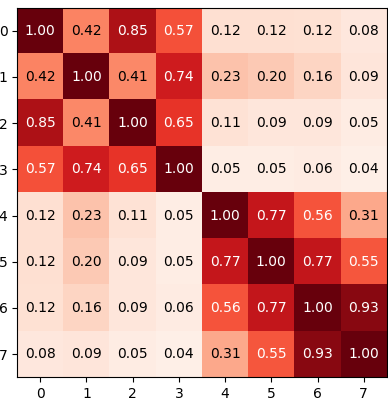
\includegraphics[width = 160pt]{img/pearson_correlation/z-normalization_non_pulsar.png}}  \\
        \end{tabular}
    \end{center}
\end{figure}

Both raw features and z-normalized features heatmaps highlight the presence of strong correlation between some pairs of features. In particular between features:

\begin{enumerate}
    \item (0) Mean of the integrated profile - (2) Excess kurtosis of the integrated profile.
    \item (1) StDev of the integrated profile - (3) Skewness of the integrated profile.
    \item (4) Mean of the DM-SNR curve - (5) Standard deviation of the DM-SNR curve.
    \item (6) Excess kurtosis of the DM-SNR curve - (7) Skewness of the DM-SNR curve.
\end{enumerate}

In general, the first four features appear to be related to each other and this is because they are all measures of the integrated profile.
The same consideration applies to the last four features, while the first four and the last four present little correlation.
The presence of correlation between features suggests that some models, such as diagonal MVG classifiers, might benefit from the application of PCA to reduce the amount of features.
Applying PCA effectively reduces the overall feature correlation, below the heatmap obtained after the application of PCA to 4 dimensions is shown: \\

\begin{figure}[H]
    \caption{Pearson correlation heatmap - PCA features}
    \begin{center}
        \begin{tabular}{ccc}
            \hspace*{-65pt}
            \subfloat[Whole dataset]{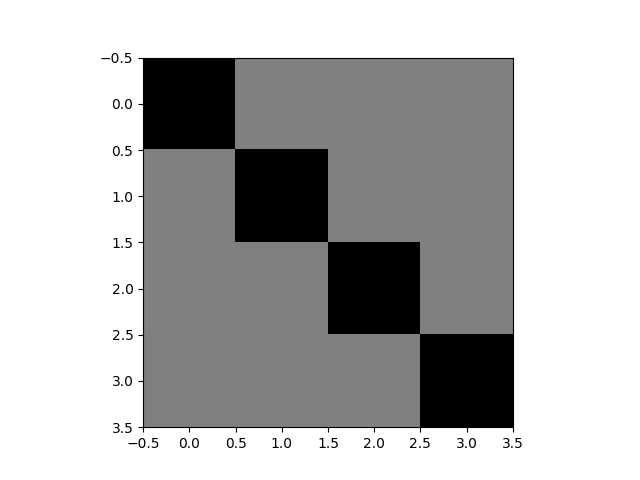
\includegraphics[width = 160pt]{img/pearson_correlation/pca_heatmap.png}} &
            \subfloat[Pulsars]{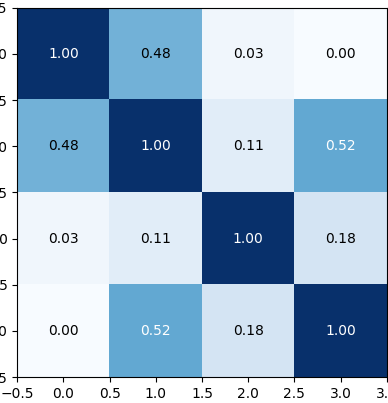
\includegraphics[width = 160pt]{img/pearson_correlation/pca_pulsar.png}}        &
            \subfloat[Non-pulsars]{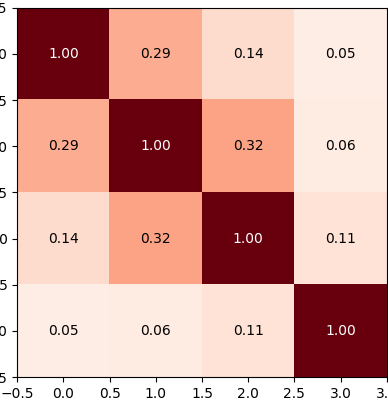
\includegraphics[width = 160pt]{img/pearson_correlation/pca_non_pulsar.png}}  \\
        \end{tabular}
    \end{center}
\end{figure}

\clearpage

\subsection{Applications}

Given no prior knowledge of the environment in which the final model will work,
3 different applications have been considered, one where the priors are balanced and two where the prior is biased towards one of the classes:
\begin{itemize}
    \item ( \(\tilde{\pi}\), Cfp, Cfn) = (0.5, 1, 1)
    \item ( \(\tilde{\pi}\), Cfp, Cfn) = (0.1, 1, 1)
    \item ( \(\tilde{\pi}\), Cfp, Cfn) = (0.9, 1, 1)
\end{itemize}

\section{Data preprocessing}

\subsection{K-fold cross-validation}

The K-fold approach has been used instead of the single-split validation technique to achieve more robust results, as the time required for K-fold is not excessive.
Models are compared by means of the Minimum Detection Cost function, a measure of the cost paid for making optimal decisions on the validation set. \\

The original training set has been split into 10 folds of similar size using the K-fold cross-validation technique.
At each iteration of the K-fold cross-validation algorithm, 9 folds have been employed for training and 1 for validation.
The data preprocessing techniques have been applied to the data after it was split into folds,
i.e. the transformation to be applied, e.g. PCA projection matrix, has been computed on the 9 train folds, then it has been applied to both training and validation folds.
This was done to avoid bias in the results, as splitting after preprocessing would have meant classifying data that the model had already seen.
\\ \\The procedure followed to train each model is the same:
\begin{enumerate}
    \item Divide training samples into K-folds, eventually applying preprocessing techniques (Computation performed only once)
    \item For each fold:
          \begin{itemize}
              \item Train a new model on the K-1 training folds
              \item Use the trained model to score the validation fold
          \end{itemize}
    \item Combine the scores of all folds
    \item Use the scores to compute minimum detection cost
\end{enumerate}

\subsection{Shuffling}

Before applying any preprocessing technique, the training dataset has been randomly shuffled to avoid any bias that could be introduced by the order of the samples.

\subsection{Z-Normalization}

All samples have been processed by means of Z-normalization, i.e. each feature has been transformed to have zero mean and unit variance.
$ x_i = \frac{x_i - \mu}{\sigma} $
$\mu$ and $\sigma$ are respectively the mean and the standard deviation of each feature describing the samples.

\subsection{Feature Gaussianization}

As an alternative preprocessing step to z-normalization, raw features have been "Gaussianized", i.e. their distributions have been transformed to be more similar to Gaussian distributions.
The Guasianization of a feature consists in computing a rank for each sample with respect to all samples and then computing the inverse of the cumulative distribution function of the standard normal distribution.
The rank of both training and evaluation data is computed with respect to the training data only.
\begin{figure}[H]
    \begin{center}
        \hspace*{-25pt}
        \begin{tabular}{ccc}
            \subfloat[]{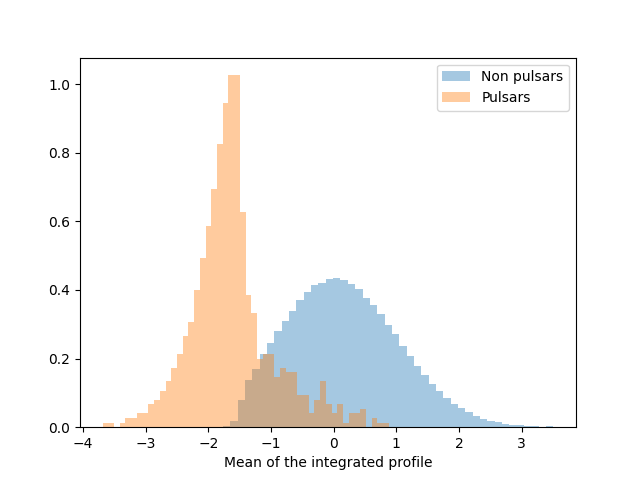
\includegraphics[width = 200pt]{img/gaussianized_features/mean_of_ip}}                    &
            \subfloat[]{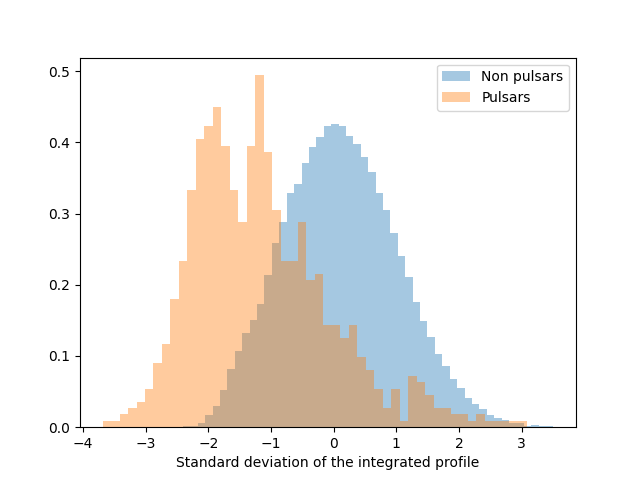
\includegraphics[width = 200pt]{img/gaussianized_features/stdev_of_ip.png}}                 \\
            \subfloat[]{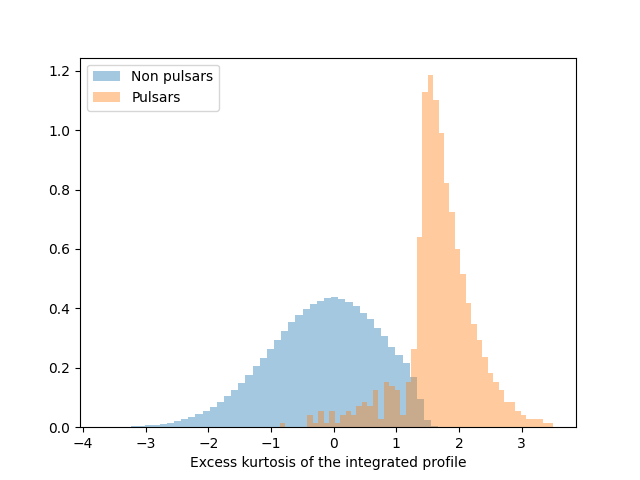
\includegraphics[width = 200pt]{img/gaussianized_features/excess_kurtosis_of_ip.png}}     &
            \subfloat[]{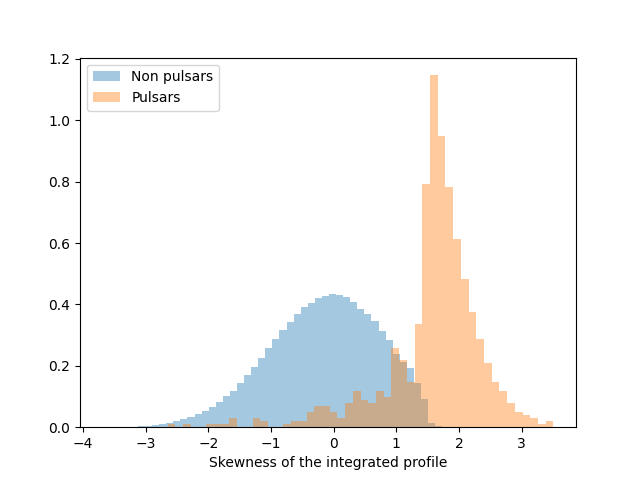
\includegraphics[width = 200pt]{img/gaussianized_features/skewness_of_ip.png}}              \\
            \subfloat[]{\includegraphics[width = 200pt]{img/gaussianized_features/mean_of_dm-snr}}                &
            \subfloat[]{\includegraphics[width = 200pt]{img/gaussianized_features/stdev_of_dm-snr.png}}             \\
            \subfloat[]{\includegraphics[width = 200pt]{img/gaussianized_features/excess_kurtosis_of_dm-snr.png}} &
            \subfloat[]{\includegraphics[width = 200pt]{img/gaussianized_features/skewness_of_dm-snr.png}}          \\
        \end{tabular}
    \end{center}
\end{figure}
Gaussianization is computed over the whole training set, therefore class-conditional distributions might still not behave like a Gaussian distribution.
This effect is clearly visible in the plots above, non-pulsars follow more regular distributions (due to their higher number of samples), while pulsars show in most cases moderate deviations from the Gaussian assumptions.
Nonetheless, the new Gaussian-like distributions are likely to improve results of classifiers that assume data are Normal distributed.
This preprocessing step also helps reducing the negative effects of the outliers as they have been mapped as "closer" values on the tail-end of the Gaussian distributions.

\subsection{Linear Discriminant Analysis}
Linear Discriminant Analysis (LDA) is deemed not useful as a preprocessing step for this dataset as LDA is capable of finding at most c - 1 discriminant directions, where c is the number of classes.
Being this a binary classification problem, the maximum number of directions LDA can produce is 1.
Given the huge loss of information this would imply, results obtained on LDA-preprocessed data will likely be worse than the ones of other approaches.
Therefore, the use of LDA is not explored in this project.

\subsection{Principal Component Analysis}

The results from the correlation analysis suggest that some models might benefit from applying a dimensionality reduction technique such as PCA to obtain uncorrelated features.
Removing correlation between features could also improve model performances by helping to reduce overfitting.
Although, given the already small number of features, further reducing it might lead to a loss of information higher than the gain obtained by the removal of correlation.
The PCA projection matrix has been computed on the training dataset and applied to the training and evaluation datasets.

\clearpage

\begin{multicols}{2}
    {
        \noindent
        \begin{addmargin}[0em]{1em}
            The effects of different values of the hyperparameter m (number of components) for PCA have been evaluated by means of minimum DCF over different MVG models.
            Table 2 shows the results obtained with different values of m, types of Gaussian classifiers, and applications.
            Full diagonal models performances worsen as the number of components decreases but overall this deterioration is not excessive.
            Classifiers with diagonal covariance on the other hand slightly improve their performances as correlated features are removed, but their overall performance is worse than the full covariance models, meaning that the training dataset is large enough to reliably estimate the full covariance matrix and effectively capture the correlation in the data.
            Since full covariance models are capable of capturing these correlations it doesn't bring any advantage to reduce the dimensionality of the data. PCA is therefore not used in the following experiments.
        \end{addmargin}
    }
    {
        \noindent
        \renewcommand{\arraystretch}{1.2}
        \begin{tabular}{cccc}

            Model      & \(\tilde{\pi}\)=0.5  & \(\tilde{\pi}\)=0.1   & \(\tilde{\pi}\)=0.9   \\ [0.5ex]

            \hline
            \multicolumn{4}{c}{RAW Features - No PCA}                                         \\
            \hline
            Full Cov.  & 0.141                & 0.280                 & 0.680                 \\
            Diagonal   & 0.194                & 0.314                 & 0.723                 \\
            Tied Full  & {\color{red} 0.113 } & {\color{blue} 0.224 } & {\color{blue} 0.571 } \\
            Tied Diag. & 0.161                & 0.266                 & 0.591                 \\

            \hline
            \multicolumn{4}{c}{RAW Features - PCA (m = 7)}                                    \\
            \hline
            Full Cov.  & 0.174                & 0.302                 & 0.708                 \\
            Diagonal   & 0.220                & 0.628                 & 0.833                 \\
            Tied Full  & {\color{red} 0.153 } & {\color{blue} 0.280 } & {\color{blue} 0.612 } \\
            Tied Diag. & 0.172                & 0.306                 & 0.639                 \\

            \hline
            \multicolumn{4}{c}{RAW Features - PCA (m = 6)}                                    \\
            \hline
            Full Cov.  & 0.172                & 0.315                 & 0.662                 \\
            Diagonal   & 0.220                & 0.645                 & 0.818                 \\
            Tied Full  & {\color{red} 0.156 } & {\color{blue} 0.288 } & {\color{blue} 0.602 } \\
            Tied Diag. & 0.173                & 0.310                 & 0.618                 \\

            \hline
            \multicolumn{4}{c}{RAW Features - PCA (m = 5)}                                    \\
            \hline
            Full Cov.  & 0.183                & 0.423                 & 0.748                 \\
            Diagonal   & 0.203                & 0.607                 & 0.797                 \\
            Tied Full  & {\color{red} 0.179 } & {\color{blue} 0.315 } & {\color{blue} 0.592 } \\
            Tied Diag. & 0.187                & 0.345                 & 0.604                 \\

            \hline
            \multicolumn{4}{c}{RAW Features - PCA (m = 4)}                                    \\
            \hline
            Full Cov.  & 0.186                & 0.434                 & 0.683                 \\
            Diagonal   & 0.199                & 0.603                 & 0.799                 \\
            Tied Full  & {\color{red} 0.172 } & {\color{blue} 0.316 } & {\color{blue} 0.601 } \\
            Tied Diag. & 0.184                & 0.347                 & 0.611                 \\
        \end{tabular}
        \captionof{table}{MVG Classifiers - Tuning of PCA components}
    }
\end{multicols}

\section{Classification}

\subsection{Gaussian models}

\subsubsection{Multivariate Gaussian Classifier}
The MVG classifier uses full covariance matrices, i.e. a covariance matrix and a mean is estimated for each classes.
Given the large number of training samples, this kind of model is expected to provide good results compared to the other types of Gaussian classifiers.

\subsubsection{Tied Gaussian Classifier}
The tied MVG model uses the same covariance matrix for all classes.
This assumption shouldn't benefit the pulsar classification problem as the training set contains a good number of samples allowing covariance matrices to be reliably estimated for each class.

\subsubsection{Naive Bayes Gaussian Classifier}
The naive Bayes MVG model simplifies the estimation by assuming that the features are independent.
We thus expect the MVG classifier with naive Bayes assumption to perform worse that the previously seen
models because the correlation heatmaps highlighted a strong correlation between features.

\subsubsection{Tied Naive Bayes Gaussian Classifier}
The tied naive Bayes MVG combines the assumptions of feature independence and tied covariance matrices.
Given that the Naive assumption is not met, this model is also expected to have some among the worst performances.

\clearpage

\subsubsection{Results}

\begin{multicols}{2}
    {

        \begin{addmargin}[0em]{1em}
            As expected Diagonal models obtain the worst performances.
            Contrary to expectations though, tied covariance models provide better results than full covariance ones.
            This could be due to the fact that since the classes represent the same physical phenomena the covariance matrices of the two classes might be similar.
            Another possible explanation could be that linear separation rules, such as the one found by the tied model, are more appropriate than quadratic ones for this classification problem.

            Raw and Z-normalized features perform similarly.
            Gaussianized features improve the performances of the diagonal covariance model but overall perform worse than the Raw and Z-normalized features on the other models.

            \(\tilde{\pi}\) = 0.9 produces the worst results, \(\tilde{\pi}\) = 0.1 provides mediocre outputs but the best ones are obtained for application \(\tilde{\pi}\) = 0.5.
            The best performances are given by the Tied Full Covariance model on the Z-Normalized Features.
        \end{addmargin}
    }
    {
        \noindent
        \renewcommand{\arraystretch}{1.2}
        \begin{tabular}{@{}cccc@{}}
            Model      & \(\tilde{\pi}\)=0.5  & \(\tilde{\pi}\)=0.1   & \(\tilde{\pi}\)=0.9  \\ [0.5ex]

            \hline
            \multicolumn{4}{c}{RAW Features}                                                 \\
            \hline
            Full Cov.  & 0.141                & 0.280                 & 0.680                \\
            Diagonal   & 0.194                & 0.314                 & 0.723                \\
            Tied Full  & {\color{red} 0.113 } & {\color{red} 0.224 }  & 0.571                \\
            Tied Diag. & 0.161                & 0.267                 & 0.591                \\

            \hline
            \multicolumn{4}{c}{Z-Normalized Features}                                        \\
            \hline
            Full Cov.  & 0.141                & 0.280                 & 0.680                \\
            Diagonal   & 0.194                & 0.314                 & 0.723                \\
            Tied Full  & {\color{red} 0.113 } & {\color{red} 0.224 }  & 0.571                \\
            Tied Diag. & 0.161                & 0.267                 & 0.591                \\

            \hline
            \multicolumn{4}{c}{Gaussianized Features}                                        \\
            \hline
            Full Cov.  & 0.154                & 0.245                 & 0.717                \\
            Diagonal   & 0.152                & 0.277                 & 0.602                \\
            Tied Full  & 0.132                & {\color{blue} 0.237 } & {\color{red} 0.532 } \\
            Tied Diag. & 0.163                & 0.292                 & 0.622                \\
        \end{tabular}
        \captionof{table}{MVG Classifiers - Comparison of results}
    }
\end{multicols}

\subsection{Logistic Regression}

The logistic regression model is trained by minimizing the sum of the logistic loss over all samples.
The L-BFGS algorithm has been used as numerical solver to find the minimum.
The logistic regression model makes no assumptions on data distribution but requires a hypothesis
on the shape of the separation rule to find. A linear separation surface has been assumed: \[ w^T x+b \]
Where w is a vector perpendicular to the separation surface and b is a bias that tells where on w the separation rule lies.

To handle class unbalance, a prior-weighted regularized version of the objective function has been used: \\

\begingroup{
\setlength{\thinmuskip}{0mu}
\hspace*{-30pt}
$J(w, b)=\frac{\lambda}{2}\|w\|^2+\frac{\pi_T}{n_T} \sum\limits_{i=\left.1\right| c_i=1 }^n \log \left(1+e^{-z_i (w^Tx_i+b)}\right)+\frac{1-\pi_T}{n_F} \sum\limits_{i=\left.1\right| c_i=0 }^n \log \left(1+e^{-z_i (w^Tx_i+b)}\right)$ \\ \\
}\endgroup
\(\lambda\) is the regularization coefficient, \(\pi_T\) is the prior probability of the positive class, \(n_T\) is the number of positive samples, \(n_F\) is the number of negative samples, \(c_i\) is the class of the \(i\)-th sample.

\subsubsection{Hyperparameter tuning: \(\lambda\)}

Small values of \(\lambda\) lead to poor generalization, while higher values of \(\lambda\) allow finding small values of \(\|w\|\) but worse separation rules.
To find the best value of \(\lambda\) the minDCF has been plotted for different applications and values of \(\lambda\) on a logarithmic scale.
For the purpose of evaluating different values of \(\lambda\), only the main application was considered (\(\pi_T = \frac{1}{2}\))

\begin{figure}[H]
    \begin{center}
        \hspace*{-25pt}
        \begin{tabular}{ccc}
            \includegraphics[width = 200pt]{img/evaluation_plots/lambda-lr-z-normalized.png} &
            \includegraphics[width = 200pt]{img/evaluation_plots/lambda-lr-gaussianized.png}   \\
        \end{tabular}
    \end{center}
\end{figure}

The best results are obtained with \(\lambda = 0 \) for all the applications, and both Z-Normalized Gaussianized features.
The reason why regularization is not helpful can be found in the small number of dimensions, which implies little risk of overfitting.
Even if regularization provides little to no improvements, in the following experiments \(\lambda\) has been set to \(10^{-6}\).

\clearpage

\subsubsection{Results}

\begin{center}
    \renewcommand{\arraystretch}{1.2}
    \begin{tabular}{@{}cccc@{}}
        Model                                                    & \(\tilde{\pi}\)=0.5   & \(\tilde{\pi}\)=0.1  & \(\tilde{\pi}\)=0.9   \\ [0.5ex]

        \hline
        \multicolumn{4}{c}{RAW Features}                                                                                                \\
        \hline
        Logisitc Regression \((\lambda = 10^{-6}, \pi_T = 0.5)\) & {\color{blue} 0.116 } & 0.219                & {\color{blue} 0.530 } \\
        Logisitc Regression \((\lambda = 10^{-6}, \pi_T = 0.1)\) & {\color{blue} 0.114 } & {\color{red} 0.213 } & 0.538                 \\
        Logisitc Regression \((\lambda = 10^{-6}, \pi_T = 0.9)\) & {\color{blue} 0.118 } & 0.218                & 0.534                 \\

        \hline
        \multicolumn{4}{c}{Z-normalized Features}                                                                                       \\
        \hline
        Logisitc Regression \((\lambda = 10^{-6}, \pi_T = 0.5)\) & {\color{blue} 0.116 } & 0.219                & {\color{blue} 0.530 } \\
        Logisitc Regression \((\lambda = 10^{-6}, \pi_T = 0.1)\) & {\color{red} 0.113 }  & {\color{red} 0.213 } & 0.537                 \\
        Logisitc Regression \((\lambda = 10^{-6}, \pi_T = 0.9)\) & 0.120                 & 0.220                & 0.537                 \\

        \hline
        \multicolumn{4}{c}{Gaussianized Features}                                                                                       \\
        \hline
        Logisitc Regression \((\lambda = 10^{-6}, \pi_T = 0.5)\) & 0.126                 & 0.238                & 0.534                 \\
        Logisitc Regression \((\lambda = 10^{-6}, \pi_T = 0.1)\) & 0.128                 & 0.229                & 0.537                 \\
        Logisitc Regression \((\lambda = 10^{-6}, \pi_T = 0.9)\) & 0.127                 & 0.238                & {\color{red} 0.524 }  \\

        \hline
        \multicolumn{4}{c}{Other models}                                                                                                \\
        \hline
        MVG Tied Full Covariance                                 & {\color{red} 0.113 }  & 0.224                & 0.571                 \\
    \end{tabular}
    \captionof{table}{Logistic Regression - Comparison of results}
\end{center}

Gaussianized features perform worse than Z-normalized and Raw features, as Logistic Regression doesn't require assumptions on the distribution of the data.
Table 4 shows that changing the value of \(\pi_T\) has little effect on the results.
Once again \(\tilde{\pi}\) = 0.9 performs worse than \(\tilde{\pi}\) = 0.1, which in turn has worse performances than \(\tilde{\pi}\) = 0.5.
Best results are obtained for Z-normalized features, with \(\pi_T = 0.1\) and \(\tilde{\pi} = 0.5\).
The improvement of using \(\pi_T = 0.1\) instead of \(\pi_T = 0.5\) is very small, but this can be explained by the unbalance in the dataset towards non-pulsar samples.
Tied MVG with full covariance has similar performances to the best logistic regression model.

\subsection{Support Vector Machines}

The SVM problem was solved using its dual formulation: \\

\begin{center}
    $ \max_{\alpha} \alpha^T1-\frac{1}{2}\alpha^TH\alpha $ subject to $ 0\leq\alpha_i\leq C_i, i=1,..,n $
\end{center}

An updated version of the constraints has also been considered to handle the unbalance between the classes.
Constraints have been changed to use costs proportional to the priors defined by the application:
$ C_T = C \cdot \frac{\pi_T}{\pi_T^{emp}} $
$ C_F = C \cdot \frac{\pi_F}{\pi_F^{emp}} $
where $ C_i = C_T $ for pulsars and $ C_i = C_F $ for non-pulsar samples.
$\pi_T^{emp}$ and $\pi_F^{emp}$ are the empirical priors obtained from the training set.


\subsubsection{Hyperparameter tuning: C}
C represents the tradeoff between having good accuracy on the training set and finding a large margin (better generalization).
To find the best value of C, K-fold cross-validation has been employed to plot the minDCF for different applications and different values of C on a logarithmic scale:

\begin{figure}[H]
    \begin{center}
        \hspace*{-25pt}
        \begin{tabular}{ccc}
            \includegraphics[width = 200pt]{img/evaluation_plots/C-svm-z-normalized-unbalanced.png} &
            \includegraphics[width = 200pt]{img/evaluation_plots/C-svm-z-normalized-balanced.png}     \\
        \end{tabular}
    \end{center}
\end{figure}
\begin{figure}[H]
    \begin{center}
        \hspace*{-25pt}
        \begin{tabular}{ccc}
            \includegraphics[width = 200pt]{img/evaluation_plots/C-svm-gaussianized-unbalanced.png} &
            \includegraphics[width = 200pt]{img/evaluation_plots/C-svm-gaussianized-balanced.png}     \\
        \end{tabular}
    \end{center}
\end{figure}

Low values of C show the models start to underfit, while high values of C clearly show signs of overfitting.
The best results are obtained with C $\approx 10^{-1}$ for both balanced ($\pi_T = 0.5$) and unbalanced applications, and for both z-normalized and gaussianized features.

\subsubsection{Results}

Minimum DCF has been computed for different values of \(\pi_T\) and \(\tilde{\pi}\) for both z-normalized and gaussianized features.
Where $ \pi_T $ is the prior probability for the true hypothesis with which the model is trained and $ \tilde{\pi} $ represents the effective prior in the context where the model will be used.

\begin{center}
    \renewcommand{\arraystretch}{1.2}
    \begin{tabular}{@{}cccc@{}}
        Model                                        & \(\tilde{\pi}\)=0.5   & \(\tilde{\pi}\)=0.1  & \(\tilde{\pi}\)=0.9  \\ [0.5ex]

        \hline
        \multicolumn{4}{c}{RAW Features}                                                                                   \\
        \hline
        Linear SVM (C = $10^{-1}$, unbalanced)       & 0.629                 & 0.803                & 0.954                \\
        Linear SVM (C = $10^{-1}$, $\pi_T = 0.5$)    & 0.592                 & 0.972                & 0.936                \\
        Linear SVM (C = $10^{-1}$, $\pi_T = 0.1$)    & 0.714                 & 1.000                & 0.931                \\
        Linear SVM (C = $10^{-1}$, $\pi_T = 0.9$)    & 0.599                 & 0.847                & 0.939                \\

        \hline
        \multicolumn{4}{c}{Z-normalized Features}                                                                          \\
        \hline
        Linear SVM (C = $10^{-1}$, unbalanced)       & 0.117                 & 0.222                & 0.584                \\
        Linear SVM (C = $10^{-1}$, $\pi_T = 0.5$)    & {\color{blue} 0.113 } & 0.223                & 0.558                \\
        Linear SVM (C = $10^{-1}$, $\pi_T = 0.1$)    & {\color{red} 0.111 }  & {\color{red} 0.214 } & 0.570                \\
        Linear SVM (C = $10^{-1}$, $\pi_T = 0.9$)    & 0.128                 & 0.234                & 0.527                \\

        \hline
        \multicolumn{4}{c}{Gaussianized Features}                                                                          \\
        \hline
        Linear SVM (C = $10^{-1}$, unbalanced)       & 0.135                 & 0.239                & 0.531                \\
        Linear SVM (C = $10^{-1}$, $\pi_T = 0.5$)    & 0.120                 & 0.251                & {\color{red} 0.519 } \\
        Linear SVM (C = $10^{-1}$, $\pi_T = 0.1$)    & 0.133                 & 0.237                & 0.531                \\
        Linear SVM (C = $10^{-1}$, $\pi_T = 0.9$)    & 0.130                 & 0.244                & 0.525                \\

        \hline
        \multicolumn{4}{c}{Other models}                                                                                   \\
        \hline
        MVG Tied Full Cov.                           & 0.113                 & 0.224                & 0.571                \\
        Log Reg \((\lambda = 10^{-6}, \pi_T = 0.1)\) & 0.113                 & 0.213                & 0.537                \\
    \end{tabular}
    \captionof{table}{Linear SVM - Comparison of results}
\end{center}

Table 5 shows that balancing classes has little impact on the outcome.
Raw features are the worst-performing ones, while z-normalized features perform better than gaussianized ones.
Best results are obtained for the z-normalized features with $\pi_T = 0.1$, \(\tilde{\pi}\) = 0.5, these are very close to the ones obtained for the best MVG and Logistic Regression models.

\subsubsection{Support Vector Machines with Polynomial Kernel}

The polynomial kernel $K(x_i, x_j) = (x_i^Tx_j + c)^d$ was used to train a linear separation surface in the expanded feature space, which corresponds to a quadratic separation rule in the original feature space.
Hyperparameters C and c were jointly optimized using a grid search, d was set to 2.

\begin{figure}[H]
    \begin{center}
        \hspace*{-25pt}
        \begin{tabular}{ccc}
            \includegraphics[width = 200pt]{img/evaluation_plots/polynomial-svm-z-normalized-C-c.png} &
            \includegraphics[width = 200pt]{img/evaluation_plots/polynomial-svm-gaussianized-C-c.png}   \\
        \end{tabular}
    \end{center}
\end{figure}
\vspace{-20pt}
\noindent
The polynomial kernel yields the best results when used with C=1 and c=0.1 for the z-normalized features and C=1, c=1 for the gaussianized features. \\

\renewcommand{\arraystretch}{1.2}
\begin{tabular}{@{}cccc@{}}
    Model                                      & \(\tilde{\pi}\)=0.5  & \(\tilde{\pi}\)=0.1  & \(\tilde{\pi}\)=0.9  \\ [0.5ex]

    \hline
    \multicolumn{4}{c}{Z-normalized Features}                                                                       \\
    \hline
    Polynomial Kernel (c = 0.1, Unbalanced)    & 0.133                & 0.246                & 0.666                \\
    Polynomial Kernel (c = 0.1, $\pi_T = 0.5$) & {\color{red} 0.103 } & {\color{red} 0.220 } & {\color{red} 0.525 } \\
    Polynomial Kernel (c = 0.1, $\pi_T = 0.1$) & 0.129                & 0.228                & 0.662                \\
    Polynomial Kernel (c = 0.1, $\pi_T = 0.9$) & 0.141                & 0.297                & 0.594                \\

    \hline
    \multicolumn{4}{c}{Gaussianized Features}                                                                       \\
    \hline
    Polynomial Kernel (c = 1, Unbalanced)      & 0.147                & 0.262                & 0.638                \\
    Polynomial Kernel (c = 1, $\pi_T = 0.5$)   & 0.128                & 0.255                & 0.570                \\
    Polynomial Kernel (c = 1, $\pi_T = 0.1$)   & 0.136                & 0.244                & 0.634                \\
    Polynomial Kernel (c = 1, $\pi_T = 0.9$)   & 0.207                & 0.485                & 0.603                \\
\end{tabular}
\captionof{table}{Polynomial Kernel SVM - Comparison of results}

\vspace*{10pt}
The best results are obtained for the Z-normalized features, with c = 0.1, \(\pi_T = 0.5\), and \(\tilde{\pi}\)=0.5.
The polynomial Kernel finds better results than any previous model but the difference is not significant.

\subsubsection{Support Vector Machines with RBF Kernel}

The RBF kernel $K(x_i, x_j) = e^{-\gamma||x_i - x_j||^2}$ requires estimating the hyperparameter $\gamma$ jointly with the hyperparameter C, this was performed using a grid search.
\begin{figure}[H]
    \begin{center}
        \hspace*{-25pt}
        \begin{tabular}{ccc}
            \includegraphics[width = 200pt]{img/evaluation_plots/rbf-svm-z-normalized-C-gamma.png} &
            \includegraphics[width = 200pt]{img/evaluation_plots/rbf-svm-gaussianized-C-gamma.png}   \\
        \end{tabular}
    \end{center}
\end{figure}

\vspace{-20pt}
\noindent
The RBF kernel has been used with C=$10^2$, $\gamma=0.1$ for both z-normalized and Gaussianized features. \\

\begin{center}
    \renewcommand{\arraystretch}{1.2}
    \begin{tabular}{@{}cccc@{}}
        Model                                    & \(\tilde{\pi}\)=0.5   & \(\tilde{\pi}\)=0.1   & \(\tilde{\pi}\)=0.9  \\ [0.5ex]

        \hline
        \multicolumn{4}{c}{Z-normalized Features}                                                                       \\
        \hline
        RBF Kernel ($\gamma$ = 0.1, Unbalanced)  & 0.121                 & {\color{blue} 0.211 } & 0.867                \\
        RBF Kernel ($\gamma = 0.1, \pi_T = 0.5$) & {\color{blue} 0.115 } & 0.236                 & 0.642                \\
        RBF Kernel ($\gamma = 0.1, \pi_T = 0.1$) & 0.123                 & {\color{blue} 0.211 } & 0.830                \\
        RBF Kernel ($\gamma = 0.1, \pi_T = 0.9$) & 0.220                 & 0.690                 & 0.630                \\

        \hline
        \multicolumn{4}{c}{Gaussianized Features}                                                                       \\
        \hline
        RBF Kernel ($\gamma$ = 0.1, Unbalanced)  & 0.120                 & {\color{red} 0.206 }  & 0.770                \\
        RBF Kernel ($\gamma = 0.1, \pi_T = 0.5$) & {\color{red} 0.109 }  & 0.219                 & 0.631                \\
        RBF Kernel ($\gamma = 0.1, \pi_T = 0.1$) & 0.121                 & {\color{red} 0.206 }  & 0.773                \\
        RBF Kernel ($\gamma = 0.1, \pi_T = 0.9$) & 0.201                 & 0.460                 & {\color{red} 0.604 } \\
    \end{tabular}
    \captionof{table}{RBF Kernel SVM - Comparison of results}
\end{center}

The best results are obtained for the Gaussianized features, with $\gamma$ = 0.1, \(\pi_T = 0.5\), and \(\tilde{\pi}\)=0.5.
Using different priors is effective in providing somewhat better results for different applications.
The RBF Kernel finds slightly worse results than the polynomial kernel.

\subsection{Gaussian Mixture Models}

GMM is a generative approach that can approximate generic distributions.
The GMMs have been estimated by iteratively applying the LBG algorithm to duplicate the number of components and the Expectation Maximization algorithm to estimate the parameters of each component.

\subsubsection{Hyperparameter tuning: number of components}

Full-covariance, diagonal-covariance, and tied-covariance models have been considered.
The performances of models with a varying number of components have been evaluated using the minDCF metric through K-fold cross-validation.
For simplicity only application $\tilde{\pi}$=0.5 has been considered.

\begin{figure}[H]
    \caption{GMM Components Evaluation}
    \begin{center}
        \begin{tabular}{ccc}
            \hspace*{-65pt}
            \includegraphics[width = 160pt]{img/evaluation_plots/gmm-components-full-covariance.png} &
            \includegraphics[width = 160pt]{img/evaluation_plots/gmm-components-tied-covariance.png} &
            \includegraphics[width = 160pt]{img/evaluation_plots/gmm-components-diagonal-covariance.png} \\
        \end{tabular}
    \end{center}
\end{figure}

The model with full covariance matrix shows signs of overfitting for 16 components and above, while tied and diagonal covariance models are capable of handling a higher number of components.
Experiments show that the best number of components is: 8 for the full-covariance model and 32 for both the tied-covariance and diagonal-covariance models.
Z-normalized features obtain better results than gaussianized ones.

\subsubsection{Results}

Minimum DCF values have been computed for: different applications, feature preprocessing, and different types of models, using the best number of components found in the previous section.

\begin{center}
    \renewcommand{\arraystretch}{1.2}
    \begin{tabular}{@{}cccc@{}}
        Model                                        & \(\tilde{\pi}\)=0.5  & \(\tilde{\pi}\)=0.1   & \(\tilde{\pi}\)=0.9  \\ [0.5ex]

        \hline
        \multicolumn{4}{c}{RAW Features}                                                                                   \\
        \hline
        GMM Full Cov. 8 components                   & 0.130                & 0.245                 & 0.630                \\
        GMM Tied Cov. 32 components                  & 0.147                & 0.297                 & 0.715                \\
        GMM Diag. Cov. 32 components                 & 0.162                & 0.288                 & 0.659                \\
        GMM Tied Diag. Cov. 32 components            & 0.159                & 0.300                 & 0.691                \\

        \hline
        \multicolumn{4}{c}{Z-normalized Features}                                                                          \\
        \hline
        GMM Full Cov. 8 components                   & {\color{red} 0.118 } & {\color{red} 0.224 }  & {\color{red} 0.562 } \\
        GMM Tied Cov. 32 components                  & 0.129                & 0.250                 & 0.615                \\
        GMM Diag. Cov. 32 components                 & 0.142                & 0.276                 & 0.599                \\
        GMM Tied Diag. Cov. 32 components            & 0.153                & 0.291                 & 0.647                \\

        \hline
        \multicolumn{4}{c}{Gaussianized Features}                                                                          \\
        \hline
        GMM Full Cov. 8 components                   & 0.128                & 0.230                 & 0.680                \\
        GMM Tied Cov. 32 components                  & 0.139                & {\color{blue} 0.226 } & 0.668                \\
        GMM Diag. Cov. 32 components                 & 0.151                & 0.284                 & 0.662                \\
        GMM Tied Diag. Cov. 32 components            & 0.184                & 0.293                 & 0.672                \\

        \hline
        \multicolumn{4}{c}{Other models}                                                                                   \\
        \hline
        MVG Tied Full Cov.                           & 0.113                & 0.224                 & 0.571                \\
        Log Reg \((\lambda = 10^{-6}, \pi_T = 0.1)\) & 0.113                & 0.213                 & 0.537                \\
        Linear SVM (C = $10^{-1}$, $\pi_T = 0.1$)    & 0.111                & 0.214                 & 0.570                \\
    \end{tabular}
    \captionof{table}{GMM - Comparison of results}
\end{center}

Diagonal models perform worse than any other model, due to the dataset being large enough to reliably estimate full covariance matrices.
Even if using more components, tied models perform worse than non-tied full covariance models, this could be due to data being split into a few large clusters rather than many small ones.
As confirmed by all other previous approaches, \(\tilde{\pi}\) = 0.5 yields better results than \(\tilde{\pi}\) = 0.1 and \(\tilde{\pi}\) = 0.9.
Overall z-normalized features produce the best results, this could be due to the reduced discriminability of clusters after applying Gaussianization.
Best results are obtained for the full covariance model with 8 components, z-normalized features, and $\tilde{\pi} = 0.5$.
The best-performing GMM model finds slightly worse results than any other model previously evaluated.


\subsection{Model selection}

The experiments highlighted that the best performing models are:
{\noindent
\begin{tabular}{@{}cccc@{}}
    Model                                                  & \(\tilde{\pi}\)=0.5 & \(\tilde{\pi}\)=0.1 & \(\tilde{\pi}\)=0.9 \\
    \hline
    MVG Tied Full Covariance                               & 0.113               & 0.224               & 0.571               \\
    Linear Log Reg $(\lambda = 10^{-6}, \pi_T = 0.1)$      & 0.113               & 0.213               & 0.537               \\
    Linear SVM (C = $10^{-1}$, $\pi_T = 0.1$)              & 0.111               & 0.214               & 0.570               \\
    Polynomial kernel SVM (C = 1, c = 0.1, $\pi_T = 0.5$)  & 0.103               & 0.220               & 0.525               \\
    RBF kernel SVM (C=$10^2$, $\gamma=0.1$, $\pi_T = 0.5$) & 0.109               & 0.219               & 0.631               \\
    GMM Full Cov. 8 components                             & 0.118               & 0.224               & 0.562               \\
\end{tabular}
}

If a single model had to be chosen based on these results, SVM with polynomial kernel would be the best choice, as it yields the best results across various applications.
However, given the additional complexity required by the quadratic model and the minimal difference in performance, Linear Logistic regression is to be preferred due to its lower complexity.
The trade-off between False Negative Rate and False Positive Rate has been plotted in the DET graph below:

\begin{center}
    \includegraphics[width=300pt]{img/evaluation_plots/DET_plot_best_models.png}
\end{center}

The Linear SVM performs better than the other models for low values of FPR, while the SVM with polynomial kernel is to be preferred if a small FNR is required.

\clearpage

Models have been so far evaluated using minimum DCF, which measures the cost of performing optimal decisions.
Now the actual cost of the decisions taken by the classifiers is measured using the Actual DCF metric.
To evaluate the difference between the two metrics, Bayes error plots have been computed for the selected models:

\begin{figure}[H]
    \begin{center}
        \hspace*{-25pt}
        \begin{tabular}{ccc}
            \includegraphics[width = 200pt]{img/bayes/bayes-error-plot-mvg.png} &
            \includegraphics[width = 200pt]{img/bayes/bayes-error-plot-lr.png}    \\
        \end{tabular}
    \end{center}
\end{figure}

\begin{figure}[H]
    \begin{center}
        \hspace*{-25pt}
        \begin{tabular}{ccc}
            \includegraphics[width = 200pt]{img/bayes/bayes-error-plot-polynomial-kernel-svm.png} &
            \includegraphics[width = 200pt]{img/bayes/bayes-error-plot-rbf-kernel-svm.png}         \\
        \end{tabular}
    \end{center}
\end{figure}

\begin{figure}[H]
    \begin{center}
        \hspace*{-25pt}
        \begin{tabular}{ccc}
            \includegraphics[width = 200pt]{img/bayes/bayes-error-plot-svm.png} &
            \includegraphics[width = 200pt]{img/bayes/bayes-error-plot-gmm.png}   \\
        \end{tabular}
    \end{center}
\end{figure}

The Gaussian Mixture Model is already well-calibrated for a large number of applications.
The MVG, SVM with polynomial kernel, and Logistic regression models present small but significant miscalibration for negative values of prior log-odds and large miscalibration errors for positive values of prior log-odds.
The linear SVM and the SVM with RBF kernel are largely miscalibrated over the whole range of applications with the only exception of small positive values of the prior log odds for the SVM models using a kernel.

\subsection{Score recalibration}

Scores of each model have been recalibrated by training a model with probabilistic interpretation using the scores as a feature.
A prior-weighted version of Logistic Regression has been used to perform the recalibration, $\tilde{\pi} = 0.5$ was used as the target application as this is expected to provide good calibration results for a wide range of applications.
Given the low risk of overfitting due to the presence of a single dimension (the scores themselves), regularization has not been employed, i.e. $\lambda = 0$.
The training set was split using the K-fold approach, at each iteration a LR model has been trained and used to score the validation fold, the scores have been then recalibrated by subtracting the prior log-odds of the target application, $\log{(\frac{\tilde{\pi}}{1-\tilde{\pi}})}$.
Below the results obtained using calibrated scores are shown.

\begin{figure}[H]
    \begin{center}
        \hspace*{-25pt}
        \begin{tabular}{ccc}
            \includegraphics[width = 200pt]{img/bayes/recalibrated-mvg.png} &
            \includegraphics[width = 200pt]{img/bayes/recalibrated-lr.png}    \\
        \end{tabular}
    \end{center}
\end{figure}

\begin{figure}[H]
    \begin{center}
        \hspace*{-25pt}
        \begin{tabular}{ccc}
            \includegraphics[width = 200pt]{img/bayes/recalibrated-polynomial-kernel-svm.png} &
            \includegraphics[width = 200pt]{img/bayes/recalibrated-rbf-kernel-svm.png}          \\
        \end{tabular}
    \end{center}
\end{figure}

\begin{figure}[H]
    \begin{center}
        \hspace*{-25pt}
        \begin{tabular}{ccc}
            \includegraphics[width = 200pt]{img/bayes/recalibrated-svm.png} &
            \includegraphics[width = 200pt]{img/bayes/recalibrated-gmm.png}   \\
        \end{tabular}
    \end{center}
\end{figure}

Overall the recalibration process has improved the performace of the models for a wide range of applications, only high values of prior log-odds are still slightly miscalibrated.

\section{Experimental results}

Data has been pre-processed with Z-normalization and Gaussianization techniques.
The two transformations have been computed on the training set and then applied to both training and test sets.

The best-performing models on the validation data have been re-trained using the entire training set to evaluate their behavior on the test set.
For each model the following steps have been performed:
\begin{itemize}
    \item The training set was split with K-fold cross-validation
    \item Each validation fold has been scored using a model trained on the training folds (preprocessing techniques have been applied at each iteration)
    \item The whole set of produced scores has been used as a feature to train a prior-weighted Logistic Regression model for the application $\tilde{\pi} = 0.5$
    \item The LR model was used to estimate a linear transformation of the scores which corresponds to the log-likelihood ratio of the two classes:
          $ f(s) = \alpha s + \beta = \log{\frac{f_{S|C}(s|H_1)}{f_{S|C}(s|H_0)}}$
    \item The original classifier has then been trained on the whole training set
    \item The test samples have been scored by the classifier
    \item The score of each test sample has been recalibrated as:\\ $s_{calibrated} = \alpha s + \beta = \alpha s + \beta' - \log{(\frac{\tilde{\pi}}{1-\tilde{\pi}})}$
\end{itemize}

Minimum DCFs and Actual DCFs have been computed for each model to evaluate if the proposed models are the best ones also for the test set. \\

{
\hspace{-58pt}
\begin{tabular}{@{}c@{}c@{\hspace{3pt}}c@{}@{}c@{\hspace{3pt}}c@{}@{}c@{\hspace{3pt}}c@{}}
    Model                                         & MinDCF                                  & ActDCF                                  & MinDCF                                  & ActDCF & MinDCF & ActDCF \\
    \hline
                                                  & \multicolumn{2}{c}{$\tilde{\pi} = 0.5$} & \multicolumn{2}{c}{$\tilde{\pi} = 0.1$} & \multicolumn{2}{c}{$\tilde{\pi} = 0.9$}                            \\
    \hline
    MVG Tied Full Covariance                      & 0.110                                   & 0.115                                   & 0.207                                   & 0.222  & 0.591  & 0.613  \\
    Linear Log Reg $(\lambda=10^{-6}, \pi_T=0.1)$ & 0.110                                   & 0.113                                   & 0.199                                   & 0.219  & 0.530  & 0.574  \\
    Linear SVM (C=$10^{-1}$, $\pi_T=0.1$)         & 0.112                                   & 0.116                                   & 0.202                                   & 0.215  & 0.549  & 0.576  \\
    Polynomial SVM (C=1, c=0.1, $\pi_T=0.5$)      & 0.105                                   & 0.108                                   & 0.199                                   & 0.215  & 0.430  & 0.461  \\
    RBF SVM (C=$10^2$, $\gamma=0.1$, $\pi_T=0.5$) & 0.111                                   & 0.112                                   & 0.231                                   & 0.246  & 0.574  & 0.658  \\
    GMM Full Cov. 8 components                    & 0.110                                   & 0.114                                   & 0.218                                   & 0.223  & 0.586  & 0.601  \\
\end{tabular}
\captionof{table}{Results on the test set}
}

\vspace*{20pt}
All models achieve very good performances for applications $\tilde{\pi} = 0.5$ and $\tilde{\pi} = 0.1$.
Overall the results are consistent with the observations made on the validation set.
SVM with polynomial kernel is confirmed as the best model,
while it provides minimal improvements with respect to other models for the balanced application,
its superiority is more evident in unbalanced environments such as $\tilde{\pi} = 0.9$.

\subsection{Multivariate Gaussian classifiers}

To evaluate if the proposed solution is the best one also for the test set,
Minimum and Actual DCFs have been computed on the test and compared with the results obtained for the validation set.

\begin{center}
    \renewcommand{\arraystretch}{1.2}
    \begin{tabular}{c|ccc|ccc}

        Model      & \(\tilde{\pi}\)=0.5            & \(\tilde{\pi}\)=0.1      & \(\tilde{\pi}\)=0.9  & \(\tilde{\pi}\)=0.5  & \(\tilde{\pi}\)=0.1  & \(\tilde{\pi}\)=0.9   \\ [0.5ex]

        \hline
                   & \multicolumn{3}{c|}{Validation} & \multicolumn{3}{c}{Test}                                                                                              \\

        \hline
        \multicolumn{7}{c}{RAW Features - No PCA}                                                                                                                           \\
        \hline
        Full Cov.  & 0.141                          & 0.280                    & 0.680                & 0.140                & 0.283                & 0.646                 \\
        Diagonal   & 0.194                          & 0.314                    & 0.723                & 0.185                & 0.330                & 0.621                 \\
        Tied Full  & {\color{red} 0.113 }           & {\color{red} 0.224 }     & 0.571                & {\color{red} 0.110 } & {\color{red} 0.207 } & 0.591                 \\
        Tied Diag. & 0.161                          & 0.266                    & 0.591                & 0.152                & 0.262                & {\color{blue} 0.544 } \\

        \hline
        \multicolumn{7}{c}{RAW Features - PCA (m = 7)}                                                                                                                      \\
        \hline
        Full Cov.  & 0.174                          & 0.302                    & 0.708                & 0.161                & 0.301                & 0.664                 \\
        Diagonal   & 0.220                          & 0.628                    & 0.833                & 0.217                & 0.626                & 0.678                 \\
        Tied Full  & 0.153                          & 0.280                    & 0.612                & 0.147                & 0.268                & 0.622                 \\
        Tied Diag. & 0.172                          & 0.306                    & 0.639                & 0.163                & 0.308                & 0.631                 \\

        \hline
        \multicolumn{7}{c}{RAW Features - PCA (m = 6)}                                                                                                                      \\
        \hline
        Full Cov.  & 0.172                          & 0.315                    & 0.662                & 0.157                & 0.309                & 0.626                 \\
        Diagonal   & 0.220                          & 0.645                    & 0.818                & 0.215                & 0.648                & 0.687                 \\
        Tied Full  & 0.156                          & 0.288                    & 0.602                & 0.147                & 0.268                & 0.607                 \\
        Tied Diag. & 0.173                          & 0.310                    & 0.618                & 0.166                & 0.309                & 0.602                 \\

        \hline
        \multicolumn{7}{c}{Z-Normalized Features}                                                                                                                           \\
        \hline
        Full Cov.  & 0.141                          & 0.280                    & 0.680                & 0.140                & 0.283                & 0.646                 \\
        Diagonal   & 0.194                          & 0.314                    & 0.723                & 0.185                & 0.330                & 0.621                 \\
        Tied Full  & {\color{red} 0.113 }           & {\color{red} 0.224 }     & 0.571                & {\color{red} 0.110 } & {\color{red} 0.207 } & 0.591                 \\
        Tied Diag. & 0.161                          & 0.267                    & 0.591                & 0.152                & 0.262                & {\color{blue} 0.544 } \\

        \hline
        \multicolumn{7}{c}{Gaussianized Features}                                                                                                                           \\
        \hline
        Full Cov.  & 0.154                          & 0.245                    & 0.717                & 0.151                & 0.241                & 0.622                 \\
        Diagonal   & 0.152                          & 0.277                    & 0.602                & 0.154                & 0.285                & 0.574                 \\
        Tied Full  & 0.132                          & {\color{blue} 0.237 }    & {\color{red} 0.532 } & 0.125                & 0.221                & {\color{red} 0.540 }  \\
        Tied Diag. & 0.163                          & 0.292                    & 0.622                & 0.158                & 0.301                & 0.568                 \\
    \end{tabular}
    \captionof{table}{Experimental results - MVG classifiers}
\end{center}

The results are consistent with those obtained during validation, as they lead to the same conclusions:
The MVG model with tied covariance remains the best performing one;
PCA leads to a slight degradation in performance;
Gaussianization obtains worse results than z-normalized features.

\subsection{Logistic Regression}

The effects of different values of the regularization parameter \(\lambda\) have been evaluated on the test set through the minimum DCF metric, and compared with the results obtained on validation data.

\begin{figure}[H]
    \begin{center}
        \hspace*{-25pt}
        \begin{tabular}{ccc}
            \includegraphics[width = 200pt]{img/evaluation_plots/evaluation-comparison-lr-z-normalized.png} &
            \includegraphics[width = 200pt]{img/evaluation_plots/evaluation-comparison-lr-gaussianized.png}   \\
        \end{tabular}
    \end{center}
\end{figure}

\vspace*{-20pt}
As for the validation set, regularization doesn't seem effective. Models have been re-trained with \(\lambda = 10^{-6}\). \\

\renewcommand{\arraystretch}{1.2}
\begin{tabular}{c|c@{\hspace{5pt}}c@{\hspace{5pt}}c|c@{\hspace{5pt}}c@{\hspace{5pt}}c}

    Model                                        & \(\tilde{\pi}\)=0.5                & \(\tilde{\pi}\)=0.1          & \(\tilde{\pi}\)=0.9   & \(\tilde{\pi}\)=0.5  & \(\tilde{\pi}\)=0.1  & \(\tilde{\pi}\)=0.9   \\ [0.5ex]

    \hline
                                                 & \multicolumn{3}{c|}{Validation set} & \multicolumn{3}{|c}{Test set}                                                                                               \\
    \hline
    \multicolumn{7}{c}{RAW Features}                                                                                                                                                                               \\
    \hline
    Log Reg \((\lambda = 10^{-6}, \pi_T = 0.5)\) & {\color{blue} 0.116 }              & 0.219                        & {\color{blue} 0.530 } & {\color{red} 0.107 } & {\color{red} 0.199 } & 0.542                 \\
    Log Reg \((\lambda = 10^{-6}, \pi_T = 0.1)\) & {\color{blue} 0.114 }              & {\color{red} 0.213 }         & 0.538                 & 0.110                & {\color{red} 0.199 } & 0.530                 \\
    Log Reg \((\lambda = 10^{-6}, \pi_T = 0.9)\) & {\color{blue} 0.118 }              & 0.218                        & 0.534                 & 0.116                & 0.205                & 0.529                 \\

    \hline
    \multicolumn{7}{c}{Z-normalized Features}                                                                                                                                                                      \\
    \hline
    Log Reg \((\lambda = 10^{-6}, \pi_T = 0.5)\) & {\color{blue} 0.116 }              & 0.219                        & {\color{blue} 0.530 } & {\color{red} 0.107 } & {\color{red} 0.199 } & 0.542                 \\
    Log Reg \((\lambda = 10^{-6}, \pi_T = 0.1)\) & {\color{red} 0.113 }               & {\color{red} 0.213 }         & 0.537                 & 0.110                & {\color{red} 0.199 } & 0.530                 \\
    Log Reg \((\lambda = 10^{-6}, \pi_T = 0.9)\) & 0.120                              & 0.220                        & 0.537                 & 0.115                & 0.203                & 0.509                 \\

    \hline
    \multicolumn{7}{c}{Gaussianized Features}                                                                                                                                                                      \\
    \hline
    Log Reg \((\lambda = 10^{-6}, \pi_T = 0.5)\) & 0.126                              & 0.238                        & 0.534                 & 0.122                & 0.215                & {\color{blue} 0.485 } \\
    Log Reg \((\lambda = 10^{-6}, \pi_T = 0.1)\) & 0.128                              & 0.229                        & 0.537                 & 0.125                & 0.211                & 0.504                 \\
    Log Reg \((\lambda = 10^{-6}, \pi_T = 0.9)\) & 0.127                              & 0.238                        & {\color{red} 0.524 }  & 0.123                & 0.212                & {\color{red} 0.484 }  \\
\end{tabular}
\captionof{table}{Experimental results - Logistic Regression}

The results are close to the ones obtained in the validation phase.
The best minDCF values on the test set are obtained for \(\pi_T = 0.5 \) rather than with the proposed \(\pi_T = 0.1 \) but the difference in performance is very small.

\subsection{Linear Support Vector Machines}

Hyperparameter C has been re-tuned on the test set, values of minDCF have been plotted in the graphs below.

\begin{figure}[H]
    \begin{center}
        \hspace*{-25pt}
        \begin{tabular}{ccc}
            \includegraphics[width = 200pt]{img/evaluation_plots/evaluation-linear-svm-z-normalized-unbalanced.png} &
            \includegraphics[width = 200pt]{img/evaluation_plots/evaluation-linear-svm-z-normalized-balanced.png}    \\
            \includegraphics[width = 200pt]{img/evaluation_plots/evaluation-linear-svm-gaussianized-unbalanced.png} &
            \includegraphics[width = 200pt]{img/evaluation_plots/evaluation-linear-svm-gaussianized-balanced.png}     \\
        \end{tabular}
    \end{center}
\end{figure}

C $\approx 10^{-1}$ was selected for all applications and types of features during validation, the same value of C remains effective also on the test set.

\subsection{Support Vector Machines with Polynomial kernel}

A grid search of parameters C and c for the polynomial kernel SVM has been performed on the test set, comparisons with validation data are reported below.

\begin{figure}[H]
    \begin{center}
        \hspace*{-25pt}
        \begin{tabular}{ccc}
            \includegraphics[width = 200pt]{img/evaluation_plots/evaluation-polynomial-svm-z-normalized.png} &
            \includegraphics[width = 200pt]{img/evaluation_plots/evaluation-polynomial-svm-gaussianized.png}   \\
        \end{tabular}
    \end{center}
\end{figure}

Validation data demonstrated that C=1 and c=0.1 were good choices for the z-normalized features and C=1, c=1 for the Gaussianized features.
Evaluation data shows that choosing $C=10^{-1}$ could have been a slightly better choice for both types of features. \\ \\

{
    \renewcommand{\arraystretch}{1.2}
    \begin{tabular}{@{}c|c@{\hspace{5pt}}c@{\hspace{5pt}}c|c@{\hspace{5pt}}c@{\hspace{5pt}}c@{}}

        Model                                  & \(\tilde{\pi}\)=0.5                & \(\tilde{\pi}\)=0.1          & \(\tilde{\pi}\)=0.9  & \(\tilde{\pi}\)=0.5  & \(\tilde{\pi}\)=0.1  & \(\tilde{\pi}\)=0.9  \\ [0.5ex]

        \hline
                                               & \multicolumn{3}{c|}{Validation set} & \multicolumn{3}{c}{Test set}                                                                                             \\
        \hline

        \multicolumn{7}{c}{Z-normalized Features}                                                                                                                                                              \\
        \hline
        Polynomial Kernel (c=0.1, $\pi_T=0.5$) & {\color{red} 0.103 }               & {\color{red} 0.220 }         & {\color{red} 0.525 } & {\color{red} 0.105 } & {\color{red} 0.199 } & {\color{red} 0.430 } \\
        Polynomial Kernel (c=0.1, $\pi_T=0.1$) & 0.129                              & 0.228                        & 0.662                & 0.124                & 0.207                & 0.605                \\
        Polynomial Kernel (c=0.1, $\pi_T=0.9$) & 0.141                              & 0.297                        & 0.594                & 0.176                & 0.570                & 0.503                \\

        \hline
        \multicolumn{7}{c}{Gaussianized Features}                                                                                                                                                              \\
        \hline
        Polynomial Kernel (c=1, $\pi_T=0.5$)   & 0.128                              & 0.255                        & 0.570                & 0.119                & 0.233                & 0.487                \\
        Polynomial Kernel (c=1, $\pi_T=0.1$)   & 0.136                              & 0.244                        & 0.634                & 0.127                & 0.228                & 0.523                \\
        Polynomial Kernel (c=1, $\pi_T=0.9$)   & 0.207                              & 0.485                        & 0.603                & 0.140                & 0.277                & 0.498                \\
    \end{tabular}
    \captionof{table}{Experimental results - Polynomial Kernel SVM}
}

\vspace{20pt}
Experimental results for the polynomial kernel SVM showcase that c = 0.1 and $\pi_T = 0.5$ using z-normalized features is the best choice for all applications, as validation suggested.
\clearpage

\subsection{Support Vector Machines with RBF kernel}

Evaluation of hyperparameter choices for the SVM with RBF kernel has also been performed through a grid search.

\begin{figure}[H]
    \begin{center}
        \hspace*{-15pt}
        \begin{tabular}{ccc}
            \includegraphics[width = 200pt]{img/evaluation_plots/evaluation-rbf-svm-z-normalized.png} &
            \includegraphics[width = 200pt]{img/evaluation_plots/evaluation-rbf-svm-gaussianized.png} &
        \end{tabular}
    \end{center}
\end{figure}

\vspace{-15pt}
The RBF kernel has previously been used with C=$10^2$, $\gamma=0.1$ for both z-normalized and Gaussianized features.
The hyperparameter tuning on the test set reveals that $\gamma=0.1$ was a good choice but perhaps C=10 would have led to slightly better results. \\

\renewcommand{\arraystretch}{1.2}
\begin{tabular}{@{}c|c@{\hspace{5pt}}c@{\hspace{5pt}}c|c@{\hspace{5pt}}c@{\hspace{5pt}}c@{}}

    Model                                    & \(\tilde{\pi}\)=0.5                & \(\tilde{\pi}\)=0.1          & \(\tilde{\pi}\)=0.9  & \(\tilde{\pi}\)=0.5   & \(\tilde{\pi}\)=0.1   & \(\tilde{\pi}\)=0.9  \\ [0.5ex]

    \hline
                                            & \multicolumn{3}{c|}{Validation set} & \multicolumn{3}{c}{Test set}                                                                                               \\
    \hline

    \multicolumn{7}{c}{Z-normalized Features}                                                                                                                                                                  \\
    \hline
    RBF Kernel ($\gamma=0.1, \pi_T=0.5$) & {\color{blue} 0.115 }              & 0.236                        & 0.642                & {\color{blue} 0.118 } & 0.229                 & 0.595                \\
    RBF Kernel ($\gamma=0.1, \pi_T=0.1$) & 0.123                              & {\color{blue} 0.211 }        & 0.830                & 0.122                 & {\color{blue} 0.209 } & 0.838                \\
    RBF Kernel ($\gamma=0.1, \pi_T=0.9$) & 0.220                              & 0.690                        & 0.630                & 0.198                 & 0.716                 & 0.576                \\

    \hline
    \multicolumn{7}{c}{Gaussianized Features}                                                                                                                                                                  \\
    \hline
    RBF Kernel ($\gamma=0.1, \pi_T=0.5$) & {\color{red} 0.109 }               & 0.219                        & 0.631                & {\color{red} 0.111 }  & 0.231                 & 0.574                \\
    RBF Kernel ($\gamma=0.1, \pi_T=0.1$) & 0.121                              & {\color{red} 0.206 }         & 0.773                & 0.119                 & {\color{red} 0.205 }  & 0.683                \\
    RBF Kernel ($\gamma=0.1, \pi_T=0.9$) & 0.201                              & 0.460                        & {\color{red} 0.604 } & 0.176                 & 0.500                 & {\color{red} 0.545 } \\
\end{tabular}
\captionof{table}{Experimental results - RBF Kernel SVM}

\vspace{15pt}
The results for the RBF Kernel SVM are consistent with the ones obtained on the validation set. Using different priors is effective for different applications.


\subsection{Gaussian Mixture Models}

Different amounts of components have been evaluated over different kinds of GMM models for z-normalized and Gaussianized features, the results are reported in the following graphs.

\begin{figure}[H]
    \begin{center}
        \begin{tabular}{ccc}
            \hspace*{-65pt}
            \includegraphics[width = 160pt]{img/evaluation_plots/evaluation-gmm-full-covariance.png}     &
            \includegraphics[width = 160pt]{img/evaluation_plots/evaluation-gmm-diagonal-covariance.png} &
            \includegraphics[width = 160pt]{img/evaluation_plots/evaluation-gmm-tied-covariance.png}       \\
        \end{tabular}
    \end{center}
\end{figure}

\vspace{-15pt}
Z-normalized features produce the best results, as for the validation data.
The optimal number of components remains 8 for the full covariance model and 32 for the tied covariance model.
The most notable difference is the performance of the diagonal covariance model, which is better for 8 components rather than 32 as validation data suggested.

\clearpage

{
    \hspace{-30pt}
    \renewcommand{\arraystretch}{1.2}
    \begin{tabular}{@{}c|c@{\hspace{5pt}}c@{\hspace{5pt}}c|c@{\hspace{5pt}}c@{\hspace{5pt}}c@{}}

        Model                             & \(\tilde{\pi}\)=0.5                & \(\tilde{\pi}\)=0.1          & \(\tilde{\pi}\)=0.9  & \(\tilde{\pi}\)=0.5  & \(\tilde{\pi}\)=0.1  & \(\tilde{\pi}\)=0.9   \\

        \hline
                                        & \multicolumn{3}{c|}{Validation set} & \multicolumn{3}{c}{Test set}                                                                                              \\
        \hline
        \multicolumn{7}{c}{RAW Features}                                                                                                                                                                   \\
        \hline
        GMM Full Cov. 8 components        & 0.130                              & 0.245                        & 0.630                & 0.143                & 0.264                & 0.606                 \\
        GMM Tied Cov. 32 components       & 0.147                              & 0.297                        & 0.715                & 0.148                & 0.295                & 0.601                 \\
        GMM Diag. Cov. 32 components      & 0.162                              & 0.288                        & 0.659                & 0.139                & 0.313                & 0.676                 \\
        GMM Tied Diag. Cov. 32 components & 0.159                              & 0.300                        & 0.691                & 0.155                & 0.306                & 0.644                 \\

        \hline
        \multicolumn{7}{c}{Z-normalized Features}                                                                                                                                                          \\
        \hline
        GMM Full Cov. 8 components        & {\color{red} 0.118 }               & {\color{red} 0.224 }         & {\color{red} 0.562 } & {\color{red} 0.110 } & {\color{red} 0.218 } & {\color{blue} 0.586 } \\
        GMM Tied Cov. 32 components       & 0.129                              & 0.250                        & 0.615                & 0.147                & 0.279                & 0.592                 \\
        GMM Diag. Cov. 32 components      & 0.142                              & 0.276                        & 0.599                & 0.138                & 0.292                & 0.609                 \\
        GMM Tied Diag. Cov. 32 components & 0.153                              & 0.291                        & 0.647                & 0.149                & 0.296                & 0.645                 \\

        \hline
        \multicolumn{7}{c}{Gaussianized Features}                                                                                                                                                          \\
        \hline
        GMM Full Cov. 8 components        & 0.128                              & 0.230                        & 0.680                & 0.135                & 0.249                & 0.590                 \\
        GMM Tied Cov. 32 components       & 0.139                              & {\color{blue} 0.226 }        & 0.668                & 0.153                & 0.253                & 0.603                 \\
        GMM Diag. Cov. 32 components      & 0.151                              & 0.284                        & 0.662                & 0.147                & 0.264                & {\color{red} 0.575 }  \\
        GMM Tied Diag. Cov. 32 components & 0.184                              & 0.293                        & 0.672                & 0.182                & 0.307                & 0.640                 \\
    \end{tabular}
    \captionof{table}{Experimental Results - GMM}
}

\vspace{20pt}
Results obtained on the test set are in line with the ones observed during the validation phase.
The Full Covariance GMM with 8 components is confirmed to be the best-performing model.

\section{Conclusions}

Different models have been evaluated for the pulsar classification task. Overall all classifiers are able to achieve good performances.
PCA, LDA, and Gaussianization didn't provide substantial improvements while Z-normalization proved to be an effective preprocessing step.
The similarity between experimental and validation results implies that evaluation and training populations behave similarly.
The SVM with polynomial kernel was confirmed to be the best performing model by the experiments carried out on the test set.

\bibliographystyle{unsrt}
\bibliography{citations}
\end{document}